\documentclass[printed,11pt,twoside,color,cover,table]{fithesis3}
\usepackage[resetfonts]{cmap}
\usepackage[T1]{fontenc}
\usepackage[main=slovak]{babel}  
\usepackage{paratype}
\usepackage[
  toc,page
]{appendix}
\usepackage[
  backend=biber,
  style=numeric,
  citestyle=numeric-comp,
  sorting=none
]{biblatex}
\addbibresource{dip-lezdik.bib}

\newcommand{\smalltt}[1]{\small\texttt{#1}\normalsize}

\thesisload

\thesissetup{
title = {Monitorovanie záťaže a využitia výpočetných zdrojov v heterogénnom výpočetnom prostredí},
author = {Juraj Leždík},
advisor = {Mgr. Miroslav Ruda},
keywords = {cloud, monitorovanie, MetaCentrum, heterogénna infraštruktúra, Hadoop, Torque, Docker, libvirt},
gender = {m},
type = {mgr},
faculty = {fi},
date =  \the\year/\the\month/\the\day,
declaration = {Prehlasujem, že táto diplomová práca je mojím pôvodným autorským dielom, ktoré som vypracoval samostatne. Všetky zdroje a literatúru, ktoré som pri vypracovaní používal alebo z nich čerpal, v práci riadne citujem s uvedením úplného odkazu na príslušný zdroj.},
}
\thesislong{abstract}{
    abstract text}
\thesislong{thanks}{
    Dikičko}

\usepackage{csquotes}
        
\usepackage{paralist}
\usepackage{amsthm}
\usepackage{amsfonts}
\usepackage{url}
\clubpenalty=10000

\begin{document}
\chapter{Úvod}
Heterogénna infraštruktúra MetaCentra poskytuje výpočtové prostriedky pre mnohé vedecké a výskumné organizácie. Spracovávajú sa v nej veľké objemy dát. Je tvorená viac než tisíckou uzlov, ktoré sú
rozmiestnené naprieč celou
Českou republikou. Podstatou fungovania heterogénnej infraštruktúry je zdieľanie veľkého výpočtového výkonu viacerými subjektami, pre ktoré by zadováženie a prevádzkovanie vlastnej infraštruktúry predstavovalo neúmernú 
ekonomickú, personálnu a prevádzkovú záťaž. Princípom zdieľania je, že prostriedky by mali byť ideálne využívané všetkými rovnako. Nemalo by dochádzať k tomu, že jeden klient vyťaží zdroje natoľko, že 
výpočtové úlohy ostatných dostanú nepomerne malý priestor. To je možné docieliť monitorovaním využitia výpočtového výkonu a vstupno-výstupných zariadení. Ak máme informácie o tom, kto koľko využíval zdroje, 
je možné toto využitie účtovať a zároveň do budúcnosti primerane regulovať. 

Aby bolo možné správne vyvodzovať závery o zaťažení infraštruktúry, je potrebné o tom zberať údaje periodicky a kontinuálne v čase. Je potrebné sledovať parametre v pravidelných intervaloch. Každému intervalu 
prináleží hodnota, ktorá vypovedá o využití prostriedkov v danom momente. Takéto dáta sa nazývajú časové rady. Na každom z množstva uzlov môžu byť spustené desiatky úloh. O každej je
potrebné zberať viacero parametrov - vyťaženie procesora, pamäte, diskov a sieťových zariadení. To predstavuje veľké množstvo metrických údajov, ktoré je potrebné ukladať a nejakým spôsobom vyhodnocovať. 
Slúžia na to 
databázy časových rád. Prípadné účtovanie sa tiež deje v určitých pravidelných intervaloch. Je preto potrebné mať možnosť spätne dohľadať údaje o využívaní zdrojov. Uchovávať podrobné metrické dáta má výnzam na určité
obdobie. Nie je príliš potrebné vedieť ako bola infraštruktúra využitá jednou úlohou pred piatimi rokmi s presnosťou na niekoľkosekundové intervaly. Okrem toho by to predstavovalo veľké požiadavky na úložné kapacity, 
ktoré rastú vzhľadom na počet uzlov, počet úloh a čas, po ktorý sú metrické údaje zberané. Je preto žiaduce po nejakej dobe dáta agregovať do väčších celkov a tiež mazať už nazbierané podrobné časové rady.

Aby boli metrické údaje spoľahlivé, je potrebné zabezpečiť ich periodický zber. Zber metrík sa uskutočňuje pravidelným zisťovaním, ako je daný zdroj vyťažený danou technológiou. 
Aplikácia, ktorá zdroj využíva, vytvorí odpoveď a pošle ju späť zbernej aplikácií. Úlohou zbernej aplikácie je správne označiť pôvod nameraných dát určitými popisnými údajmi a odoslať tieto dáta
do centrálneho (nie však nevyhnutne centralizovaného) úložiska. Úložisko sa stará o prijímanie a uchovávanie dát z uzlov infraštruktúry a ich spravovanie, archiváciu a prípadne agregáciu historických dát.

Prostredie MetaCentra predstavuje heterogénnu infraštruktúru. Na riešenie výpočtových úloh sa použivajú rôzne technológie a aplikácie. Rôzne aplikácie pristupujú k výpočtovým problémom odlišnými postupmi,
no zároveň používajú spoločné výpočtové zdroje. Metrické dáta, ktoré budem zberať, by mali vypovedať o vyťažení tých istých druhov zdrojov. Je preto potrebné identifikovať, ktoré metrické dáta z 
jednej aplikácie je možné porovnať s údajmi z inej aplikácie. Takto môžeme dostať celkový obraz o tom, ako rôzne technológie využívajú jednu skupinu zdrojov a len takto je možné vzájomne tieto technológie 
porovnávať. 


\chapter{Heterogénna infraštruktúra MetaCentra}
Projekt MetaCentrum vznikol v roku 1996 a od roku 1999 je jeho činnosť zastrešovaná organizáciou CESNET. Zaoberá sa budovaním národnej gridovej infraštruktúry a prepojením s podobnými projektami za hranicami
Českej republiky. Projekt je oficiálnou súčasťou Európskej gridovej iniciatívy (EGI). Úlohou MetaCentra je predovšetkým koordinácia a rozširovanie infraštruktúry či už o vlastné zdroje alebo prostredníctvom
partnerov, ktorý poskytujú výpočtový výkon svojich clusterov. Jedná sa hlavne o akademickú spoluprácu. MetaCentrum spravuje výpočtové prostriedky a dátové úložiská AV, JČU, MU, MZLU, UK, VUT, ZČU.
V súčasnosti disponuje (stav k 30.7. 2010) 1500 procesorovými jadrami, 100 TB využiteľnej diskovej kapacity v podobe poľa a 400 TB kapacity v podobe pások. Služby využíva 385 registrovaných aktívnych užívateľov, ktorí 
spolu na 750 tisíc úlohách využili 7 miliónov hodín procesorového času.

MetaCentrum primárne poskytuje svoj výpočtový výkon a úložnú kapacitu. Taktiež sprístupňuje svoje programové vybavenie a vývojové prostredie a hlavne množstvo aplikácií využívaných na výskumné účely, ako napr. 
Ansys, Gaussian, Matlab, Mathematica. Taktiež sa venuje vývoju v oblasti gridového a cloudového počítania, napr. v oblasti plánovania, gridového middleware, optimalizácie a paralelizácie výpočtov a virtualizácie
infraštruktúry. Dôležitou funkciou je účasť na medzinárodných projektoch, využívanie medzinárodnej výpočtovej infraštruktúry a využívanie skúseností na rozvoj v domácom prostredí.\cite{metacentrum}

Cieľom MetaCentra je umožňiť využívať veľkú množinu výpočtových zdrojov mnohým subjektom. Infraštruktúra je rôznorodá, obsahuje rôzne typy uzlov, od jednotlivých pracovných staníc, ktoré poskytujú
časť svojho výkonu až po dedikované clustre, ktoré slúžia na riešenie zložitých výpočtových úloh. V MetaCentre je výpočtový výkon sprístupnený viacerými technológiami.
\\Prvým typom je \textit{cloud}. Jedná sa o virtualizované prostredie, kde na jednom fyzickom stroji môže byť súbežne spustených viacero nezávislých strojov.
\\Druhým typom je \textit{grid}. Grid spája mnoho uzlov aj s rôznym geografickým umiestnením do jedného výpočtového uzla, ktorý rieši náročné výpočtové úlohy. Uzly môžu poskytovať celý svoj výpočtový výkon
alebo len jeho časť.
\\MetaCentrum taktiež poskytuje užívateľom využívanie rôzneho aplikačného softvéru, prípadne softvérových nástrojov, ktoré slúžia ako medzivrstva pri riešení zložitých výpočtov. Tento druh nástrojov
sprostredkováva výkon jednotlivých uzlov podobným spôsobom ako grid a vytvára akoby jeden výkonný stroj.

\section{Kontrola zdrojov infraštruktúry}
Bez ohľadu na to, aký prístup si užívateľ zvolí k využívaniu zdieľaných výpočtových prostriedkov, jeho výpočty sa v konečnom dôsledku budú musieť realizovať na fyzickom hardvéri poskytovateľa. 
Aj keď sa daná úloha vypočítava na viacerých uzloch a rozličnými postupmi, vlastník by mal mať možnosť nejakým jednotným spôsobom určiť, ako je reálne celá infraštruktúra vyťažovaná.

\section{Cloud}
Cloud predstavuje abstraktnú výpočetnú infraštruktúru, ktorej fyzické výpočtové prostriedky sú zdieľané viacerými užívateľmi. 
Pre cloud sú typické dva koncepty:
\begin{description}
\item[\emph{Abstrakcia:}] Podrobnosti o implementácií systému sú abstrahované užívateľom a vývojárom. Aplikácie bežia na fyzických systémoch,
ktoré nie sú špecifikované, dáta sú uložené na neznámych miestach, administrácia systémov je odovzdaná iným a užívatelia majú
všestranný prístup.
\item[\emph{Virtualizácia:}] Cloud virtualizuje systémy zdieľaním zdrojov. Systémy a úložný priestor môže byť poskytovaný podľa potrieb z 
centralizovanej infraštruktúry, ceny sú stanovené na základe meraní, je možný prenájom viacerým subjektom a zdroje sú škáľovateľné podľa aktivity.
\end{description}
\cite{cloud_bible}

Prevádzkovateľ cloudu môže zvoliť rôzne prístupy k tomu, akým spôsobom bude poskytovať svoje zdroje. Tie sa dajú rozdeliť do troch kategórií:

\begin{description}
\item[\emph{Infrastructure as a Service (IaaS):}] Užívateľ má možnosť využívať zdroje cloudu podľa svojich hardvérových požiadaviek.
Môže si presne určiť koľko pamäte, procesorov alebo diskovej kapacity požaduje. Poskytovateľ služby spravuje hardvérovú infraštruktúru,
kým klient je zodpovedný za ostatné aspekty nasadenia. To zahŕňa operačný systém, aplikácie a užívateľskú interakciu so systémom. \cite{cloud_bible}
\item[\emph{Platform as a Service (PaaS):}] Prevádzkovateľ služby poskyzuje hardvér, operačný systém, aplikácie, služby, vývojové prostredia
a kontrolné štruktúry. Užívateľ môže nasadiť vlastné aplikácie na cloudovú infraštruktúru alebo využívať aplikácie, ktoré boli naprogramované
jazykmi a nástrojmi, podporovanými prevádzkovateľom. %\cite[10]{cloud_bible:1}
\item[\emph{Software as a Service (SaaS):}] Tento model sprístupňuje užívateľovi konkrétnu aplikáciu prostredníctvom tenkého klientskeho 
rozhrania (zväčša cez webový prehliadač) a zodpovednosť zákazníka spočíva len v spravovaní svojich dát a v interakcií s užívateľským systémom.\cite{cloud_bible}
\end{description}

Cloud umožňuje jednoducho spravovať a meniť výpočtový výkon, ktorý má užívateľ k dispozícií. Má to význam, ak sa rozrastú požiadavky užívateľa na výkon, alebo naopak z dôvodu obmedzenej prevádzky či 
nedostatku výpočtových úloh sa nároky môžu zmenšiť. Užívateľ môže dané prostriedky využívať hneď, bez veľkých počiatočných investicií, ktoré by si buď nemohol dovoliť, alebo ak sú výpočtové úlohy krátkodobejšieho rázu, nákup
stroja s požadovaným výkonom by bol nevhodnou investíciou. Užívateľ sa nemusí starať o nákup hardvéru, jeho zostavovanie do funkčných serverov a ich následné rozširovanie a správu. Tieto služby zabezpečuje prevádzkovateľ cloudovej infraštruktúry.
Pre neho je zase dôležité mať prehľad o tom, ako sú jeho inštalované kapacity využívané. Či už z pohľadu skvalitňovania vlastných poskytovaných služieb alebo vo vzťahu ku klientovi a k tomu, v akej miere spotrebováva poskytovaný výkon.
Výpočtové prostriedky sú poskytované viacerými spôsobmi:

\section{Realizácia konceptov cloudu}
Prostredie cloudu má za cieľ poskytovať užívateľom prostriedky variabilne vzhľadom na ich aktuálne požiadavky. Druhým dôležitým aspektom je
izolovanosť jednotlivých užívateľov v rámci celej infraštrukúry, aby prípadné probléímtak
\subsection{Virtuálne stroje}
Virtuálne stroje poskytujú úplnú virtualizáciu fyzickej hardvérovej štruktúry. Na jednom hosťujúcom počítači môže byť spustených viacero virtuálnych strojov. Každý má svoj vlastný virtuálny procesor, pamäť, grafický procesor, pevný disk 
a periférie. Operačný systém spustený vo virtuálnom stroji je izolovaný od hosťovského opračného systému (ak ho hosťovský počítač má). Takéto riešenie má jednu bezpečnostnú výhodu oproti aplikačným 
kontajnerom. Nežiadúce fungovanie jedného virtuálneho stroja neovplyvňuje beh ostatných.

\subsubsection{Hypervízor}
Hypervízor je softvér, ktorý poskytuje virtualizačné nástroje potrebné na ich izolovaný beh v rámci jedného fyzického stroja. Rozlišujeme 2 typy:
\begin{description}
\item[natívny] - na hosťujúcom počítači nie je nainštalovaný žiadny operačný systém. Hypervízor spravuje hardvér hosťujúceho počítača a kontroluje beh operačných systémov, ktoré sa javia ako procesy.
Príkladom je VMware ESX/ESXi, Oracle VM Server for x86 alebo Citrix XenServer.
\item[hosťovaný] - hypervízor je spustený ako program v operačnom systéme hosťujúceho počítača. Príkladom je QEMU, VMware Workstation alebo VirtualBox.
\end{description}
\cite{hypervisorTypes}

\subsection{Aplikačné kontajnery}
Kontajnery predstavujú odlišný prístup k virtualizácií ako virtuálne stroje. Tiež ide o snahu spúšťať softvér v prostredí oddelenom od skutočného hardvéru a operačného systému. Na rozdiel od úplných virtuálnych strojov 
nie je virtualizovaný celý hardvér, ale len softvérové vybavenie nevyhnutné na spustenie programu. Rozdiel v architektúre ilustruje nasledovný obrázok: 
\begin{figure}[h]
\begin{center}
       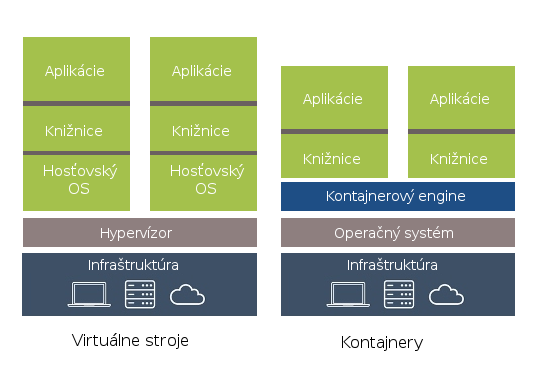
\includegraphics[width=0.8\textwidth]{images/kontajnery-virtualky.png}
       \caption{Porovnanie architektúry kontajnerov a virtuálnych strojov s natívnym hypervízorom}
\end{center}
\end{figure}
Kontajnery zdieľajú jadro operačného systému hosťovského počítača a jeho množinu prostriedkov. Jednotlivé kontajnery dostávajú kontrolovaný prístup k výpočtovému výkonu, pamäti, úložnej kapacite, 
sieti a prípadne ďalším prostriedkom. Takýto spôsob virtualizácie predstavuje zníženú záťaž na hosťujúci počítač, pretože nie je virtualizovaný celý operačný systém a ani hardvér.
\\Kontajnery môžu byť spustené aj v rámci virtuálnych strojov. Cieľom tejto práce ale nie je monitorovanie takto vnorených kontajnerov.

\section{MapReduce aplikačné prostredia}

\section{Gridové počítanie}

\section{Technológie využívané v MetaCentre}
V prostredí MetaCentra sú nasadené do produkčnej prevádzky softvéry, ktoré umožňujú využívať výkon spomínanými technológiami. Jedná sa o heterogénnu infraštruktúru, ktorú tvoria výkonné clustre ale 
aj jednotlivé uzly rozmiestnené po celej republike. Virtuálne stroje sú poskytované prostredníctvom linuxového modulu jadra \textit{KVM}. Na prácu s nimi je využívaná knižnica \textit{libvirt}. 
Na virtualizáciu v podobe kontajnerov je nasadený softvér \textit{Docker}. Technológiu distribuovaného počítania v podobe MapReduce aplikácií zabezpečuje \textit{Apache Hadoop}.
Koordináciu gridových výpočtov zabezpečuje \textit{Torque}. V nasledujúcich sekciách sa podrobnejšie venujem popisu jednotlivých softvérov.
 
\subsection{libvirt/KVM}
KVM\footnotemark\footnotetext{Kernel-based Virtual Machine} je plné virtualizačné riešenie pre Linux na x86 hardvér, obsahujúce virtualizačné rozšírenia (Intel VT or AMD-V).
Pozostáva z nahrateľného modulu jadra, kvm.ko, ktorý poskytuje základ virtualizačnej infraštruktúry a šepcifický modul, kvm-intel.ko alebo kvm-amd.ko, ktoré zabezpečujú virtuálizáciu procesora od daného výrobcu.
Je možné virtualizovať obrazy s operačnými systémami Linux, Windows, OS X alebo aj ďalšími. Každý virtuálny stroj má vlastný virtualizovaný hardvér: procesor, pamäť, sieťovú kartu, disk, grafický adaptér atď. 
KVM je open-source softvér. Virtualizačný modul jadra sa nachádza v Linuxe od verzie 2.6.20.\cite{kvm}
\\libvirt je sada nástrojov na prácu s virtualizačnými schopnosťami Linuxu (a ostatných OS). Je to voľný softvér dostupný pod licenciou GNU LGPL. 
Obsahuje API v jazyku C a väzby pre bežné programovacie jazyky, ako napr. Python, C\#, Java, Ruby alebo Go.\cite{libvirt}
\\Predstavuje vrstvu abstrakcie, ktorá zjednocuje prácu s hypervízormi od viacerých výrobcov. Umožňuje vytvoriť a zrušiť virtuálny stroj, spúšťať a vypínať, meniť jeho konfiguráciu a pridelené zdroje a tiež zisťovať údaje o využití zdrojov.

\subsection{Docker}
Docker predstavuje kontajnerový engine a sadu nástrojov, ktorá umožňuje zabaliť aplikáciu so všetkými jej závislosťami do kompaktnej jednotky (tzv. kontajnery) určenej na softvérový vývoj. Kontajnery Dockeru 
obaľujú softvér kompletným súborovým systémom, ktorý zahŕňa všetko, čo daný softvér potrebuje na spustenie: kód, nástroje potrebné na beh, systémové nástroje a knižnice. Toto zaručuje, že program bude pracovať rovnako bez ohľadu na prostredie, v ktorom
je spustený.\cite{docker} 
Pri behu jednotlivé kontajnery zdieľajú jadro operačného systému.
\\Docker rozlišuje kontajnery a obrazy. Obraz predstavuje softvérový balík so všetkými závislosťami, kontajner reprezentuje jeho beh. Preto môže existovať viacero kontajnerov, v ktorých je spustený ten istý
softvér.

\subsection{Hadoop}
Projekt Apache Hadoop vyvíja open-source softvér na spoľahlivé, škálovateľné, distribuované výpočty. Apache Hadoop je prostredie, ktoré umožňuje distribuované spracovávanie veľkých množstiev dát
naprieč clustermi, používajúcimi jednoduché programovacie modely. Je navrhnutý tak, aby bol škálovateľný od jednotlivých serverov po tisícky strojov, kde každý poskytuje lokálny výpočtový výkon a úložný priestor.
Nespolieha sa na vysokú dosupnosť hardvérových prostriedkov, ale je navrhnutý, aby detekoval a zvládal chyby na aplikačnej vrstve, takže poskytuje vysoko dostupnú službu nad clusterom počítačov, 
z ktorých každý je náchylný na chyby. \cite{hadoop}
\\Hadoop využíva MapReduce aplikačný model. Vývojárom poskytuje programovacie prostredie, ktoré uľahčuje výmenu dát medzi jednotlivými fragmetnami veľkej výpočtovej úlohy. Toto zjednodušuje
prácu spojenú s komunikáciou medzi jednotlivými uzlami a umožňuje sa viac zamerať na samotný výpočetný problém.
\\Projekt pozostáva z týchto modulov:
\begin{description}
\item[\emph{Hadoop Common:}] spoločné nástroje, ktoré podporujú ostatné Hadoop moduly
\item[\emph{Hadoop Distributed File System (HDFS™):}] distribuovaný súborový systém, ktorý poskytuje vysokú priepustnosť
\item[\emph{Hadoop YARN:}] prostredie pre plánovanie úloh a správu zdrojov clustera
\item[\emph{Hadoop MapReduce:}] systém založený na YARN pre paralelné spracovávanie veľkých množstiev dát, prostredie pre plánovanie úloh a správu zdrojov clustera
\end{description}

\subsection{PBS Professional}

\chapter{Zber a uchovávanie monitorovacích dát}
Monitorovanie akejkoľvek (nielen počítačovej) prevádzky je dôležitá oblasť, ktorá má význam pre jej správne fungovanie, správu, zdokonaľovanie a servis. Monitorovanie nám poskytuje dáta, ktoré majú viacero 
spôsobov využitia:
\begin{description}
\item[\emph{Prehľad o aktuálnom vyťažení zdrojov}]
Pri zbere dát toto zodpovedá meraniu konkrétnej hodnoty sledovaného parametru. Kvantifikáciou sledovaného zdroja dostaneme predstavu o tom, ako je používaný "teraz", čiže v prítomnosti. Môžeme tak detegovať prípadné
preťaženie zdroja, jeho dostupnosť alebo zlyhanie.
\item[\emph{Prehľad o vyťažení zdrojov za určitú dobu}]
Vyťaženie zdrojov sa v priebehu času mení. Nielen z krátkodobého hľadiska, kedy napríklad prebieha výpočet náročných úloh len v určitých hodinách, ale aj zo strednodobého (v období letných prázdnin je infraštruktúra 
vyťažovaná menej) a dlhodobého hľadiska (požiadavky na výkon sa zväčšujú). Uchovávanie monitorovacích dát predstavuje kľúčovú požiadavku, aby sme mohli sledovať, aké trendy vo využívaní mali jednotlivé sledované zdroje v priebehu nejakej doby.
Z takto nahromadených dát môžeme vypočítavať rôzne štatistiky a ďalej ich analyzovať.
\item[\emph{Prehľad o vyťažení zdrojov podľa parametrov}]
Vyťaženie zdrojov predstavuje určitú skalárnu hodnotu či už pre jednotlivé uzly alebo naprieč celou infraštruktúrou. Niekedy je však potrebné zistiť, ako boli využívané zdroje len v určitej oblasti cloudu,
alebo napr. ako boli využívané disky s kapacitou nad 1 TB. Okrem jednoduchého zberu dát o vyťažení nám dobre navhrnuté monitorovanie poskytuje aj komplexnejšie informácie, na základe ktorých je potom možné
selektívne určovať vyťaženie zdrojov. To je možné dosiahnuť zberom doplňujúcich dát pripísaných jednotlivým metrikám.
\item[\emph{Prehľad o stave zdrojov z hľadiska správy a plánovania}]
Nezanedbateľný význam má monitorovanie z hľadiska údržby a servisu poskytovaných služieb. Z dostupných dát vieme indentifikovať nefunkčný zdroj a nahradiť ho novým. V prípade vysokého vyťaženie zas môžeme vyvodiť záver, že zdroje už nie sú
dostačujúce a je potrebné ich nejakým spôsobom rozšíriť prípadne zlepšiť efektivitu ich využívania. Takisto vieme do určitej miery predpovedať, ako budú zdroje v budúcnosti využívané, čo je podstatné pri samotnom plánovaní 
odstávok, servisnej činnosti alebo dočasného rozšírenia zdrojov.
\item[\emph{Účtovanie vyťaženia zdrojov}]
Každá poskytovaná služba má svojho spotrebiteľa. Dáta o používaní zdrojov sú jediným možným spôsobom ako rozumne stanoviť cenu za používané zdroje.
Taktiež na ich základe môžeme sledovať činnosť jednotlivých užívateľov v systémoch a stanoviť im akceptovateľné podmienky na využívanie služieb.
\end{description}

\section{Všeobecné problémy monitorovania}
Problematika monitorovania v sebe zahŕňa viacero aspektov, ktoré možno oddeliť, nájsť pre ne vhodné riešenia a spojiť ich tak do funkčného celku. 

\subsection{Identifikácia relevantných metrík}
V prvom rade je potrebné identifikovať, čo vlastne potrebujeme pre konkrétny systém monitorovať. Jedná sa o určenie zdrojov kľúčových pre dané prostredie. V tomto prípade sú to údaje o vyťažení
procesorov, pamätí, sieťových rozhraní a diskov. Niektoré údaje, ktoré potrebujeme vedieť, je možné odvodiť z iných už nameraných hodnôt, napr. percentuálna miera vyťaženia procesora. 

\subsection{Analýza v reálnom čase a varovania}
Namerané hodnoty metrík je okrem neskoršej štatistickej analýzy potrebné sledovať a analyzovať v reálnom čase. Metrika môže mať svoje kritické hodnoty. Sú to hodnoty, ktoré naznačujú, že daný zdroj sa vymyká bežným očakávaniam o využití.
Na toto je vhodné reagovať. Či už sa jedná o zapísanie hlásenia do logu, zobrazenie varovania alebo prípadné zaslanie emailu či SMS správy s popisom udalosti.

\subsection{Meracie intervaly}
Ďalším čiastkovým problémom je granularita metrík. Zdroje sú kontinuálne využívané v čase. Tieto dáta je potrebné nejakým spôsobom digitalizovať. V určitom momente sa pozrieme na zdroj, kvanitifikujeme, do akej miery je využitý a danú
hodnotu zobrazíme prípadne uložíme. Meranie je po uplynutí určitého intervalu zopakovať, aby sme získali opäť aktuálne údaje. Rôzne zdroje sa menia v čase rôznou intenzitou. Napr. spotrebovaný porcesrový čas
sa mení prakticky neustále, zatiaľčo počet chýb na sieťovom rozhraní sa mení zriedkavejšie. Je preto dôležité určiť aj periodicitu zberania jednotlivých metrík. Niektoré metriky sa môžu meniť takým spôsobom, ž
e nie je efektívne sledovať ich zmenu pravidelne v nejakých intervaloch. Namiesto toho je efektívnejšie pri zmene daného parametru túto zmenu ohlásiť spolu s novou hodnotou.

\subsection{Počet zdrojov a ich identifikácia}
Množstvo zdrojov predstavuje ďalšiu oblasť, ktorú je potrebné zvážiť. Môžeme disponovať rôznym počtom zdrojov viacerých druhov, rozmiestnenými na viacerých miestach pod správou mnohých ľudí - prípadne oddelení. Metrické dáta vo svojej
podstate len kvantifikujú využitie zdroja vo všeobecnosti. Zaobchádzajú s ním v tom zmysle, ako by bol len jeden. Nehovoria nič bližšie o tom, o aký zdroj sa jedná, kde je ho možné nájsť. V rámci širšieho
systému je preto dôležitá jednoznačná identifikácia daného zdroja. O danom zdroji preto chceme zistiť napr. názov uzla, kde sa nachádza, prípadne výrobný model. Takéto údaje sa nazývajú metadáta - čiže dáta o (v tomto 
prípade o metrických) dátach.

\subsection{Ukladanie dát}
Uchovávanie metrických dát je kľúčovou sučasťou monitorovacieho systému. Doba, po ktorú vlastníci zdrojov uchovávajú metrické dáta, sa líši systém od systému. V niektorých oblastiach to je dokonca upravené zákonmi - napr. telekomunikácie,
v iných je to na zvážení majiteľa infraštruktúry. Množstvo dát, ktoré je treba uložiť, závisí od viacerých parametrov. Sú nimi počet druhov zdrojov, počet jednotlivých inštancií zdrojov, počet metrík, ktoré sa o zdrojoch
uchovávajú, periodicita zbieraných metrík a do určitej miery aj spôsob identifikácie daného zdroja. Prikladám tabuľku, ktorá ilustruje ako sa mení počet záznamov v závislosti na uvedených parametroch.
\\Ukladanie metrických dát predstavuje zároveň úzke hrdlo monitorovacieho riešenia. Zistenie hodnôt metrík pre kontrétny zdroj predstavuje v zásade serializovanú činnosť. V určitom čase sú všetky zdroje opýtané na to, ako sú vyťažené. Po jednom
zistia svoje hodnoty a odošlú ich na uloženie. Počet metrík pre jeden zdroj je v bežnej praxi len zlomkom počtu zdrojov. Na časť systému, ktorá je zodpovedná za ukladanie metrík, sú preto v pravidelných intervaloch kladené pomerne 
veľké nároky. Je ich už ale možné spracovávať paralelne. Centralizácia úložiska by znamenala prílišnú záťaž na monitorovacie uzly, preto je vhodné, aby takéto úložisko bolo distribuované a prispôsobené na paralelné spracovávanie veľkých
objemov dát.

\subsection{Vizualizácia a analýza dát}
Zozbierané metrické dáta je ďalej potrebné nejakým spôsobom zobraziť. Na to sú vhodné čiarové grafy s dvoma osami, kde horizontálna os predstavuje čas a vertikálna os predstavuje hodnotu nameranej metriky.
Analýza zozbieraných dát slúži na odhalenie trendov vo využívaní zdrojov a môže viesť k zdokonaľovaniu systému a k lepšiemu plánovaniu využívania zdrojov.

\subsection{Monitorovanie v heterogénnom výpočtovom prostredí}
V oblasti cloudového a gridového výpočtového prostredia je pre monitorovanie kľúčové sledovať vyťaženie výpočtových zdrojov. Konkrétne procesor, výpočtová pamäť, trvalý ukladací priestor a sieťová infraštruktúra. Toto je spoločné
pre všetky technológie a okrem týchto zdrojov je vhodné sledovať aj parametre špecifické pre jednotlivé oblasti. Tým sa budem konkrétne venovať v kapitole Metriky.
\\Automatizované monitorovanie výpočtového prostredia so sebou prináša aj špecifické problémy. Odvíjajú sa od toho, že monitorovanie je vykonávané strojovo (tj. pomocou počítača) a monitorované zdroje sú takisto stroje, ktorých
stav z pohľadu využitia sa mení veľmi dynamicky.
\\Rozdielny je aj prístup jednotlivých technológií v tom, ako poskytujú výpočtové zdroje. Aplikačné kontajnery a virtuálne stroje sa snažia rozdeliť celú infraštruktúru na menšie viac-menej uzavreté celky, 
ktoré sú potom sprostredkované užívateľom. Každý tento celok má pridelené zdroje, ktoré potom využíva. Množstvo týchto zdrojov je možné meniť, ale súvisí to s reštartovaním virtuálneho stroja alebo kontajnera.
\\Technológia gridu predstavuje odlišný prístup, kde z menších celkov (uzlov infraštruktúry) sú vytvárané väčšie virtuálne celky, ktoré vykonávajú výpočty.

\subsubsection{Problematika intervalov}
U vysoko výkonných výpočtových systémov sa jednotlivé operácie vykonávajú vo veľmi krátkych časových intervaloch. Rádovo sú to nanosekundy. Jednotlivé procesy a výpočtové úlohy dostávajú na krátky čas k dispozícií všetky zdroje, čím 
sa z vyššieho pohľadu zabezpečuje paralelizácia. To spôsobuje vyťaženie množstva inštancií zdrojov mnohými učastníkmi. Celkový stav infraštruktúry z pohľadu vykonaných úloh a prenesených dát sa preto mení veľmi dynamicky a je vhodné
zbierať dáta o zdrojoch v rozmedzí jednej až troch sekúnd. 
\\Nezanedbateľnú rolu hrá aj čas potrebný na získanie jedného takéhoto "snímku" využitia zdrojov. Ak zberáme metriky v intervale dvoch sekúnd, očakávame, že odpoveď príde v kratšom intervale. 
V najlepšom prípade by táto doba odpovede mala byť len malý zlomok periódy danej metriky. Táto doba je v priamej závislosti od toho, koľko subjektov infraštruktúru využíva a koľko úloh spúšťa. 
Ak je však doba odpovede dlhšia ako samotný interval zberu, je to potrebné nejako riešiť. Nie je vhodné vygenerovať ďalšiu požiadavku na "snímku". Žiaducejším spôsobom riadenia je také, ktoré počká, kým sa daná požiadavka vykoná, a potom v nasledovnom intervale je meranie vykonané znova. Týmto sa predíde nadmernej záťaži
celého systému.
\\To, ako sa systém vysporiadava z takýmto neočakávaným správaním, som zohľadňoval pri jednotlivých dostupných softvérových riešeniach.

\subsubsection{Detekcia nových zdrojov a užívateľov}
Heterogénna štruktúra v čase mení aj množstvo a kapacitu svojich poskytovaných zdrojov. Nie je možné staticky definovať zoznam procesorov, diskov, alebo virtuálnych strojov ktoré treba monitorovať. Podobne je to aj s užívateľmi. Proces
vytvárania nových užívateľov je zautomatizovaný, takisto užívatelia môžu automatizovať vykonávanie svojich výpočtových úloh. Monitorovacie riešenie sa preto musí vedieť vysporiadať s týmito dynamickými zmenami, musí ich vedieť 
automaticky detegovať a zberať o nich metrické dáta.

\section{Časové rady}
Monitorovacie dáta vo svojej podstate predstavujú časové rady.
Časová rada je sekvencia dát, kde danému časovému okamihu zodpovedá jedna hodnota. Príkladom je zaznamenávanie teplôt v priebehu roka, výšky oceánskeho prílivu alebo množstvo áut, ktoré za určitú dobu
prejde jedným bodom diaľnice. Efektívnou metódou vizuálizácie dát časových rád sú čiarové grafy. Horizontálna os reprezentuje plynutie času a na vertikálnej osi sú znázornené hodnoty v danom čase.

\subsection{Analýza časových rád}
Analýza časových rád sa primárne zaoberá získavaniu štatistík o zozbieraných dátach, napr. priemerná teplota počas celého roka. Medzi ďaľšie úlohy patrí:
\begin{description}
\item[\emph{Exploračná analýza dát}] - cieľom je detekcia vzorov v dátach. Kľúčová je grafická reprezentácia dát, ktorá môže pomôcť odhaliť súvisloti, ktoré by neboli jasné z algebraickej analýzy.\cite{eda}
\item[\emph{Aproximácia na funkciu}] - cieľom je nájsť krivku alebo matematickú funkciu, ktorá pre daný bod v čase generuje hodnotu rovnakú alebo v určitej rozumnej odchýlke od skutočnej nameranej hodnoty.
\item[\emph{Predpovedanie}] - v štatistike patrí do oblasti štatistického odvodzovania. Ide o snahu vytvoriť štatistický model, ktorý vie s určitou pravdepodobnosťou predpovedať vývoje metrík v buduúcnosti.
\item[\emph{Klasifikácia}] - ide o identifikáciu určitých javov v dátach a ich priradenie k nejakej udalosti - napr. výpadok, spúšťanie virtuálneho stroja atď.                               
\end{description}

\subsection{Zaobchádzanie s historickými dátami}
\label{sec:example}
Pri zbere časových dát je jedným z dôležitých parametrov kapacita, ktorá je potrebná na ukladanie dát. Uvažujme nasledovný príklad. Infraštruktúra má 5 000 uzlov, o každom zberáme 15 metrík každých 5 sekúnd,
označených metadátami o dĺžke 100 bajtov. Hodnota časovej zámky je reprezentovaná 4 bajtami a hodnota metriky tiež 4 bajtami. Po roku budú mať zberané dáta v nekomprimovanej podobe približe 51,1 TB. Túto kapacitu
je možné zmenšovať rôznymi kompresnými metódami a taktiež agregáciou historických dát. Tým sa myslí združovanie nameraných dát do väčších intervalov a ukladanie príslušných hodnôt za tieto dlhšie intervaly.

\chapter{Aktuálne monitorovacie riešenia}
Problematike monitorovania softvéru a infraštruktúry sa venuje viacero komerčných alebo open-source aplikácií, prípadne aplikácií zadarmo. Rôznymi technológiami riešia zber dát, ich uchovávanie, vizualizáciu a operácie nad
nimi. Najprv sa venujem popisu aplikácií, ktoré súvisia so samotným monitorovaním, neskôr rozoberám dostupné riešenia v oblasti uchovávania časových rád.

\section{Monitorovacie riešenia}
Monitorovací softvér vo všeobecnosti poskytuje ucelené monitorovacie riešenie od zberu dát, cez uchovávanie a vizualizáciu. Pri konkrétnych riešeniach sa venujem aj tomu, akým spôsobom je ich možné
rozšíriť o zber ďalších dát a ako sa správajú v prípade, že metriky nie sú dostupné v požadovaných intervaloch.

\subsection{Nagios}
Nagios je aplikácia, ktorá poskytuje komplexné riešenie na monitorovanie systémov. Poskytuje informácie o kľúčových komponentoch infraštruktúry vrátane aplikácií, služieb, operačného systému, sieťových protokolov, systémových metrík
a sieťovej infraštruktúry. \cite{nagios} 
Aplikácia pozostáva z jadra, ktoré riadi zber údajov, a z množstva pluginov tretích strán. Tie sa zaoberajú monitorovaním jednotlivých oblastí systému. Ďalej aplikácia
poskytuje grafické užívateľské rozhranie v podobe webového rozhrania. K dispozícií sú rôzne vizualizácie nameraných dát, grafy a histogramy. Nagios disponuje aj systémom užívateľských účtov. Tie sa delia na dva typy: 
administrátorov a bežných užívatešov. Bežní užívatelia majú prístup k nameraným hodnotám a zobrazovaniu grafov. Administrátori môžu konfigurovať aplikáciu, pridávať služby, ktoré je potrebné monitorovať,
upravovať parametre monitorovania a spravovať užívateľské účty. K dispozícií je aj uchovávanie konfigurácie aplikácie a spravovanie týchto konfigurácií. Súčasťou je aj systém na upozorňovanie na kritické
hodnoty, či už formou emailu alebo SMS správou. Aplikácia je vyvíjaná pre platformu CentOS a Red Hat Enterprise Linux. Namerané metriky sa uchovávajú v logovacích súboroch. 
Pomocou pluginov je možné ich odosielať do MySQL databázy prípadne PostgreSQL. 
\\Nagios predstavuje centralizované riešenie pre  monitorovanie, kde výkonné jadro riadi zberanie metrík naprieč celým systémom. 
Jadro a pluginy sú dostupné zdarma, komplexné riešenie je potrebné zakúpiť. Cena sa odvíja od množstva zariadení, ktoré je potrebné monitorovať. Zariadením sa rozumie niečo, čo má IP adresu, 
prípadne doménové meno - či už sa jedná o firewall, switch, router, pracovnú stanicu alebo server. 
\\V súčasnosti Nagios disponuje pluginmi Docker, Hadoop aj libvirt/KVM, no ani jeden z pluginov nemonitoruje požadované metriky.

\subsubsection{Rozšírenia}
Nagios pluginy existujú vo forme skriptov alebo spustiteľných programov. Aby mohli fungovať ako pluginy ich činnosť musí spĺnať dve kritériá. Prvým je výpis aspoň jedného riadku na štandardný výstup.
Ten sa týka nameraných metrík. Od verzie 3 je podporovaných aj viacerov riadkov na výstupe. Druhým kritériom je návratová hodnota.
API rozoznáva štyri návratové hodnoty. Tie zodpovedajú stavom monitorovanej služby - či je služba v poriadku, či vygenerovala nejaké varovanie, či je jej stav kritický, alebo neznámy. Prednastavená maximálna dĺžka 
výstupu je 4 kB, je ju však možé pomocou konfigurácie zmeniť.

\subsubsection{Riadenie intervalov zberu metrík}
Pre jednotlivé monitorovacie sondy je možné nadefinovať interval v počte sekúnd, v ktorom je potrebné aby sonda ukončila svoju činnosť. Ak sa tak nestane, proces sondy je ukončený a jej návratová hodnota
zaznamenaná ako kritická. Taktiež je toto zaznamenané do logov Nagiosu. Tento mechanizmus predstavuje akúsi poslednú záchranu pred zahltením systému pluginmi, ktoré sa nesprávajú podľa očakávaní.

\subsection{Icinga}
Icinga predstavuje open-source monitorovací nástroj, ktorý je nástupcom Nagiosu. Je založená na princípe paralelnej činnosti viacerých vlákien, čo poskytuje možnosť vykonávať množstvo meraní
za krátky časový interval. Zabezpečuje monitorovanie záťaže zdrojov ako disk, procesor, pamäť a sieť a to v operačných systémoch na základe Linuxu a aj v prostredí Windows. Ďalej podporuje zberanie
dát o mnohých ďalších službách, ako je monitoring databáz, odozvy serverov, webových služieb, výkonu JVM, sledovanie logov. Podporuje monitorovanie virtualizačnej platformy VMWare. 
Poskytuje aj bežné mechanizmy v oblasti monitorovania ako generovanie notifikácií o neštandardnom správaní, na ktoré je možné reagovať spustením nejakého systémové príkazu. Na ukladanie dát 
používa svoju databázu, no podporuje aj odosielanie dát do databázy časových rád InfluxDB.
\\V súčasnosti Icniga nie je schopná monitorovať ani jednu z technológií využívaných v prostredí MetaCentra.

\subsubsection{Rozšíriteľnosť aplikácie}
Icinga poskytuje systém, akým je možné do nej pridať kontroly nových metrík, prostredníctvom tzv. check príkazov. Jedná sa o kofiguračné objekty, kde užívateľ definuje príkaz,
ktorý sa má spustiť, spolu s hodnotami jeho argumentov. Icinga určí stav tejto kontroly podľa návratovej hodnoty príkazu.\cite{icinga-plugin}
Hodnoty a názvy metrík sú vracané vo forme textového výstupu.

\subsection{Zabbix}
Zabbix je open-source aplikácia na monitorovanie systémov od malých systémov s malým počtom uzlov až po veľké firemné prostredia s tisíckami strojov. Architektúra aplikácie pozostáva zo serveru a agentov.
Úlohou agentov je zber monitorovacích dát a ich odosielanie serveru. Komunikácia týchto dvoch častí môže prebiehať dvoma spôsobmi. V prvom prípade si agent vyžiada zoznam metrík, ktoré má sledovať. Následne 
serveru odosiela všetky tieto metriky po jednom. Druhou alternatívou je postup, kedy sa server agenta pýta na jednotlivé hodnoty metrík a ten mu ich odosiela. Server spravuje konfiguráciu jednotlivých agentov,
čo uľahčuje ovládanie ich správania naprieč celou infraštruktúrou.
\\Aplikácia zberá udáje o dostupných zdrojoch uzlov, o počte procesorov, dostupnej pamäti a úložnej kapacite. Taktiež zberá údaje o aktuálnom vyťažení týchto zdrojov. Okrem toho sleduje dostupnosť a parametre
služieb ako FTP, DNS, HTTP, SMTP, SSH a rôznych ďalších. Taktiež poskytuje údaje o proces bežiacich v systéme a o užívateľoch. Zaujímavým prvkom je monitorovanie logov, ich analýza a vytváranie varovaní 
v prípade, že je to nutné.
\\Zabbix vie zberané dáta vizualizovať pomocou grafov. Súčasťou je aj sledovanie zberaných hodnôt, ich kontrola na požadovaný rozsah a generovanie notifikácií. Poskytuje aj manažment užívateľov samotnej 
aplikácie a ich práv na zaobchádzanie s ňou. Zabbix podporuje autodetekciou nových prvkov v infraštruktúre. Kontroluje zadaný sieťový rozsah na nové uzly, služby na nich bežiace alebo automaticky registruje
nových spustených agentov.
\\Na zvládanie záťaže vo veľkých systémoch je zavedený systém proxy serverov. Tie zhlukujú dáta z niekoľkých agentov a až potom sú odosielané centrálnemu serveru.
\\Zabbix má vlastnú databázu na uchovávanie zozbieraných dát. Rozdeluje ich na históriu a trendy. História sú dáta tak, ako boli namerané, trendy predstavujú agregované dáta z pohľadu dlhších období, napr. v 
rádoch rokov. Tiež je možné využiť na ukladanie dát SQL databázy - MySQL, PostgreSQL, SQLite.
\\V súčasnosti Zabbix prostredníctvom stiahnuteľných modulov podporuje monitorovanie Docker kontajnerov a virtuálnych strojov.

\subsubsection{Rozšírenia}
Aplikáciu je možné rozšíriť o vlastné moduly zberajúce dáta tromi spôsobmi. 
\begin{description}
\item[\emph{užívateľské parametre}] - v tomto prípade užívateľ definuje v agentovi názov metriky a príkaz, ktorý sa má vykonať na zber jej hodnoty
\item[\emph{externé kontroly}] - jedná sa o kontrolu na strane servera, kedy je tiež definovaný skript zberajúci dáta a server ho spúšťa
\item[\emph{system.run}] - jedná sa o kontrolu na strane agenta, ktorá podporuje väčší výstup spusteného príkazu ako len hodnota metriky
\end{description}
\cite{zabbix-modules}
Okrem toho poskytuje aj programové API a vývoj vlastných modulov ako zdieľaných knižníc, ktoré musia implementovať požadované funkcie.

\subsubsection{Riadenie intervalov zberu metrík}
Konrola zberu jednotlivých metrík z hľadiska doby trvania tohoto zberu sa v Zabbixe odohráva na úrovni agenta a serveru. Na úrovni agenta ide o čas, ktorý je možné stráviť spracovávaním a získavaním
jednotlivých metrík. Pre server je potom definovaná doba, ktorú je ochotný čakať na odpoveď agenta. Tieto doby je možné konfigurovať v rozsahu od 1 do 30 sekúnd.\cite{zabbix-server}
Zabbix nespracuje jednoduchú kontrolu na hodnotu metriky, ktorá trvá dlhšie ako túto dobu.\cite{zabbix-limit}
Dokumentácia však neuvádza, ako sa aplikácia riadi beh externých procesov, ktoré zberajú dáta.

\subsection{Ganglia} 
Ganglia je škáľovateľný distribuovaný systém na monitorovanie výkonných systémov ako sú clustre a gridy. Je založená na hierarchickom návrhu 
som zameraním na federácie clusterov. Využíva bežné štandardy, ako napr. XML na reprezentáciu dát, XDR na prenos dát a RRDTool na
ukladanie a vizualizáciu dát.\cite{ganglia} 
Cieľom aplikácie je zabezpečiť čo najmenšiu nabytočnú záťaž na uzloch a vysokú
mieru súbežnosti. Ganglia vznikla na University of California v rámci Berkeley Millennium Project. Je to open-source projekt
pod licenciou BSD. V súčasnosti je nasadená na mnohých operačných systémoch a podporuje viacero procesorových architektúr.
\\Ganglia má architektúru monitorovacieho démona, ktorý je spustený na každom monitorovanom uzle, a démona, ktorý uchováva zozbierané údaje do
round-robin archívu.
K dispozícií sú aj nástroje na získanie aktuálnych údajov konkrétnej sondy a tiež webové rozhranie na zobrazovanie zaznamenaných údajov.
\\Hadoop je možné nakonfigurovať tak, aby odosielal metriky zbernému démonovi Ganglie. Ostatné integrácie v súčasnosti neobsahuje.

\subsubsection{Rozšíriteľnosť aplikácie}
K dispozícií je mnoho pzásuvných modulov v podobe skriptov operačného systému alebo programov napísaných v skriptovacích jazykoch ako Ruby,
Perl či Python. Pluginy poskytujú monitorovanie prihlásených užívateľov v systéme, rôznych aplikácií a služieb, ako napr. DNS, HTTP, ďalej
podporujú zber senzorických údajov (teplota procesora, otáčky ventilátora), monitorovanie rýchlosti siete či napr. ZFS súborového systému.\cite{ganglia-hadoop}

\subsection{AppDynamics}
AppDynamics predstavuje zaujímavé riešnie v oblasti monitorovania. Snaží sa do istej miery zjednotiť a prepojiť monitorovanie aplikácií 
a infaštruktúry a následne tak ľahšie identifikovať problémy s výkonom. Obsahuje bohaté vizualizácie nie len v podobe grafov o vyťažení,
ale aj mapy a plošné grafy pozostávajúce s uzlov prepojených čiarami, ktoré reprezentujú vyťaženie spojenia jednotlivých služieb - 
napr. webový server, databáza a servery aplikačnej logiky. Monitoruje vyťaženie zdrojov ako sú procesor, pamäť, vstupno-výstupné operácie
a sieť u jednotlivých uzlov infraštruktúry a dáva ich do súvisu s tým, aké role tieto uzly vykonávajú v danej business aplikácií.
\\Okrem toho disponuje aj integráciami s IaaS a PaaS cloudovými službami od Amazonu, RedHatu či Microsoftu a integráciami s mnohými aplikáciami
vrátane zberu metrík o zdrojoch v Hadoope a Dockeri.\cite{appdyn}
\\AppDynamics predstavuje komerčné riešenie. Verzia s obmedzeným monitorovacím záberom a s obmedzenou dĺžkou ukladania údajov je k 
dispozícií aj zdarma, plná verzia je platená.

\subsubsection{Rozšíriteľnosť aplikácie}
Nakoľko je AppDynamics komerčný softvér, rozšírenia sú k dispozícií od výrobcu. Neexistuje programové rozhranie ani iný spôsobo, napr. spúšťanie rozšírení ako samostatných programov a analýza 
ich výstupu.

\section{Ďalšie nástroje}
V súvislosti s monitorovaním existujú aj ďalšie programy a nástroje, ktoré sa dajú využiť na zber dát. Niektoré poskytujú riešenia v oblasti riadenia zberu a zápisu dát (napr. collectd), iné
sa zaoberajú riadením prístupu k zdrojom a môžu slúžiť ako zdroj dát.

\subsection{Linux cgroups}
Linux cgroups je technológia linuxového jadra, ktorá umožňuje limitovať, sledovať a izolovať spotrebu prostriedkov systému jednotlivými procesmi. Zavádza stromovo organizované kontrolné skupiny. 
Kontrolná skupina obsahuje obmedzenia pre jeden systémový prostriedok, tzv. susbsystém. Príklad subsystémov, ktoré poskytuje Red Hat Enterprise Linux: 
\begin{description}
\item[\emph{blkio}] - tento subsystém nastavuje limity na zápis a čítanie z blokových zariadení, ako napríklad HDD, SSD alebo USB disky.
\item[\emph{cpu}] - tento subsystém využíva systémový plánovač na poskytovanie prístupu k procesoru pre jednotlivé úlohy.
\item[\emph{cpuacct}] - tento subsystém generuje automatické správy o tom, koľko procesorových zdrojov využila úloha v danej skupine.
\item[\emph{cpuset}] - tento subsystém priraďuje jednotlivé procesory (na viacprocesorovom systéme) a pamäťové uzly úlohám v skupine.
\item[\emph{devices}] - tento subsystém povoľuje alebo zakazuje prístup k zariadeniam podľa úloh v skupine.
\item[\emph{freezer}] - tento subsystém zastavuje alebo obnovuje vykonávanie úloh v skupine
\item[\emph{memory}] - tento subsystém nastavuje limity na využívanie pamäte úlohami v skupine a generuje automatické správy na pamäťové zdroje použité úlohami.
\item[\emph{net\_cls}] - tento susbsystém označuje sieťové pakety identifikátorom triedy, čo umožňuje linuxovému ovládaču prevádzky identifikovať pakety, ktoré pochádzajú od konkrétnej úlohy.
\item[\emph{net\_prio}] - tento subsystém poskytuje spôsob, ako dynamicky nastavovať prioritu sieťovej prevádzky pre sieťové rozhrania.
\item[\emph{ns}] - toto je menný subsystém.
\end{description}
\cite{cgroups}

Pre každý subsystém existuje jeden strom kontrolných skupín. Ďalej skupina obsahuje zoznam procesov, ktoré podliehajú definovaným obmedzeniam. V strome kontrolných skupín sa proces vyskystuje len raz.
V cloudovom prostredí však jednotlivé technológie využívajú a spúšťajú mnoho procesov, ktoré by sa obtiažne priraďovali jednotlivým užívateľom v súvislosti so spustenými aplikáciami, preto tento spôsob
monitorovania nie je úplne vhodný. Takisto zberané metriky o subsystémoch sú agregované pre kontrolnú skupinu, tj. predstavujú súčet pre skupinu procesov, takže nie je možné jednoznačne určiť koľko zdrojov spotreboval
ten ktorý proces.

\subsection{collectd}
Collectd je open-source monitorovacia aplikácia vyvinutá v jazyku C. Má architektúru jadra a pluginov, ktoré sa starajú o mnoho činností súvisiacich s monitorovaním od zbierania dát, cez
zapisovanie metrík a sledovanie prahových hodnôt a upozorňovanie. Jadro predovšetkým ovláda a kontroluje vykonávanie týchto aktivít. V pravidelných intervaloch spúšťa kontroly metrík, 
analyzuje namerané hodnoty, generuje notifikácie v prípade, že hodnoty sú mimo požadovaný rozsah, alebo ak nedorazili 
v požadovaných intervaloch. V súčasnosti je k dispozícií viac než 90 pluginov. Poskytujú monitorovanie základných výpočtových zdrojov ako sú procesor, pamäť, disky a sieťové rozhrania, ďalej monitorovanie
mnohých aplikácií (napr. databázy, e-mail, webové servery) a protokolov. Zvolený programovací jazyk dáva dobré predpoklady na výkon a prenositeľnosť, čo umožňuje beh na systémoch bez 
skriptovacích jazykoc alebo cron démona, ako napríklad zabudované systémy. Zároveň ale disponuje optimalizáciami a prvkami, aby zvládal stovky tisíc metrík.\cite{collectd} 
\\Collectd nepodporuje vizualizáciu dát ani historickú analýzu. Nepredstavuje preto úplné monitorovacie riešenie. Samotný zápis dát je uskutočňovaný pomocou pluginov a 
teda je možné zvoliť z viacerých spôsobov uchovávania dát. V súčasnosti podporuje zápis do viacerých databáz, napr. MongoDB, OpenTSDB, alebo metódou HTTP POST či do súborov RRD. 
\\V súčasnosti obsahuje plugin pre monitorovanie libvirt/KVM.

\subsubsection{Rozšíriteľnosť aplikácie}
Collectd poskytuje viacero spôsobov, akým je možné ho rozšíriť. Prvým aspektom je zber metrík. Umožňuje zber dodatočných metrík pomocou
spúšťania systémových príkazov, pomocou rozšírení v rôznych programovacích jazykoch (Perl, Python, Java). Ďalej je možné využiť natívne
API v jazyku C. Cez toto API je možné aplikáciu rozšíriť v ohľade notifikácií, zápisu metrických dát a spôsobu logovania udalostí.

\subsubsection{Riadenie intervalov zberu metrík}
V prípade, že hodnota metriky nedorazila v požadovanom intervale, je generované hlásenie. Neprichádza k tomu ale hneď po prvej chybe. Collectd zavádza mechanizmus časových limitov.
To znamená, že meranie niekoľkokrát zopakuje v požadovanom intervale a až potom vygeneruje hlásenie s varovaním. Počet opakovaní
je možné definovať. 

\section{Databázy časových rád}
Na uchovávanie zozbierných dát sú najvhodnejšie databázy časových rád. Sú optimalizované na uchovávanie veľkého objemu dát a spracovávanie tisícok zápisov za sekundu. Vizualizácia nie je primárnou funkciou,
databázy majú buď vlastné zabudované riešenia, alebo sú poskytované ako samostatný softvér.

\subsection{OpenTSDB}
OpenTSDB je open-source databáza na uchovávanie a sprístupňovanie veľkých objemov časových dát. Pozostáva z Time Series Daemon (TSD) a z utilít pre príkazový riadok. Interakcia s OpenTSDB je primárne realizovaná cez jedného alebo viacerých TSD. Každý TSD je nezávislý.
Neexistuje žiadny riadiaci proces, žiadny zdieľaný stav, takže je možné spustiť toľko TSD, koľko je potrebné na zvládnutie požadovanej záťaže. Každý TSD používa open-source databázu HBase
na ukladanie a vyberanie dát časových rád. HBase schéma je vysoko optimalizovaná na rýchlu agregáciu podobných časových rád, aby minimalizovala požiadavky na úložný priestor. 
Používatelia TSD nemusia pristupovať do HBase priamo. S TSD je možné komunikovať cez jednoduchý protokol podobný Telnetu, cez HTTP API alebo cez jednoduché GUI. Všetka komunikácia
sa deje na tom istom porte (TSD odhadne protokol klienta pohľadom na prvých niekoľko bajtov, ktoré obdrží).\cite{openTSDB}
\\Na obrázku je znázornená architektúra OpenTSDB. Viacero démonov môže zapisovať dáta do jednej databázy, ktorá je potom distribuovaná v rámci Hadoop architektúry.
\begin{figure}[h]
\begin{center}
       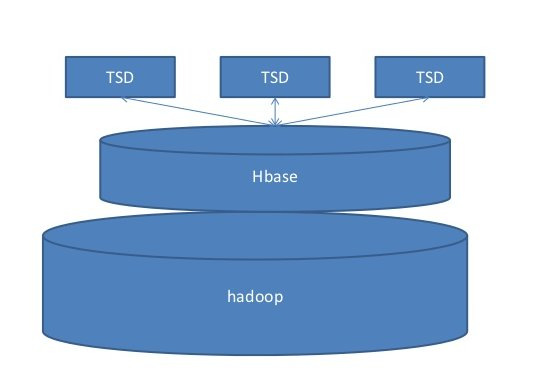
\includegraphics[width=0.8\textwidth]{images/opentsdb-arch.jpg}
       \caption{Architektúra OpenTSDB}\cite{opentsdb-arch}
\end{center}
\end{figure}
\\OpenTSDB uchováva čas zozbierania metriky, jej hodnotu a súbor popisných dát, ktoré sa nazývajú tagy. Na ich základe je potom možné
v nameraných dáta vyhľadávať, zhlukovať ich a analyzovať. Jednou z odlišností od iných databáz je, že má schopnosť uchovávať "surové" nezhlukované dáta po veľmi dlhú dobu (čiže od začiatku merania až do prítomnosti).
\\Na vizualizáciu dát existuje nástroj Grafana. Je to open-source webový engine, ktorý vytvára grafy zo zhromaždených dát. Je možné meniť časové rozpätie, za ktoré sa majú grafy metrík zobraziť.
Na obrázku je znázornených viacero metrík, ktorých názov sa nachádza v spodnej časti. Ich hodnoty sa v čase menia, čo je zachytené čiarovým grafom, kde horizontálna os predstavuje čas a vertikálna os hodnotu
metriky v tom čase.
\begin{figure}[h]
\begin{center}
       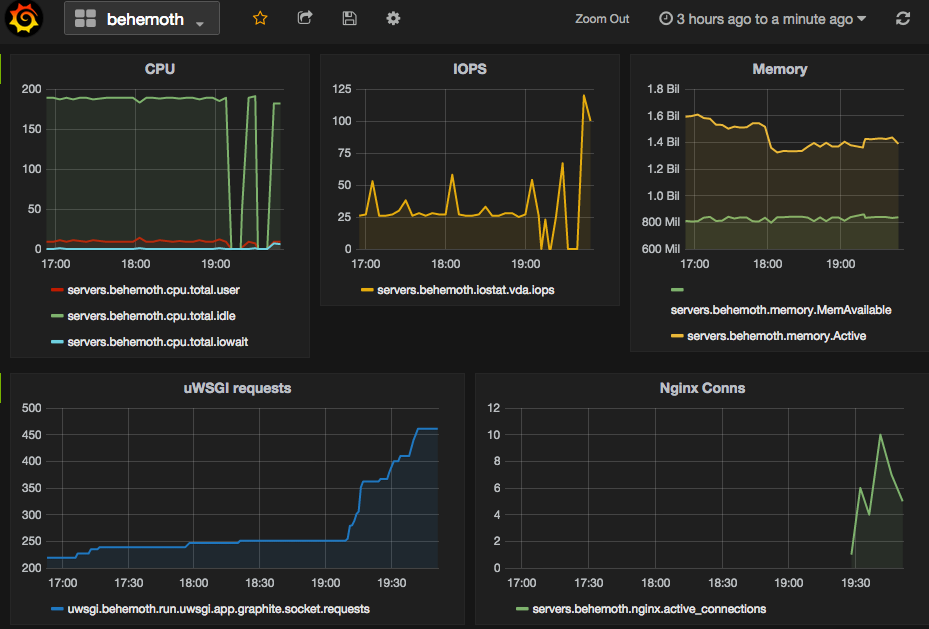
\includegraphics[width=0.8\textwidth]{images/grafana.png}
       \caption{Vizualizácia časových rád OpenTSDB nástrojom Grafana}\cite{grafana}
\end{center}
\end{figure}

\subsection{InfluxDB}
InfluxDB je platforma v jazyku Go na zbieranie, uchovávanie, vizualizáciu a správu časových dát. InfluxDB je určená na použitie ako úložisko dát v takých prípadoch, ktoré zahŕňajú veľké množstvo
dát označených časovou známkou, vrátane DevOps monitorovania, aplikačných metrík, senzorových dát internetu vecí, a na analýzu dát v reálnom čase.\cite{influxdb}
 Užívateľ môže vytvoriť viacero nezávislých databáz. 
Dáta sa zapisujú a čítajú pomocou rozhrania príkazového riadka, rôznych klientskych knižníc, alebo pomocou HTTP API. Na vizualizáciu dát používa modul \emph{chronograf}.

\subsubsection{Politiky udržiavania}
Každá databáza obsahuje pravidlá, ktoré definujú, po akú dobu majú byť ukladané dáta časových rád a koľko kópií dát má byť vytvorených. Jedna databáza môže mať niekoľko takýchto politík. Pri zápise 
do nej je môžné špecifikovať, ktorá politika sa má pre zápis použiť. Pri vytvorení databázy je automaticky vytvorená jedna politika.

\subsubsection{Kontinuálne dotazovanie a agregácia}
Databáza je schopná periodicky vykonávať požiadavky na dáta. Cieľom je zmenšovanie objemu dát. Ide o zhlukovanie dát s vysokou frekvenciou zberu, čím vzniknú dáta s menšou hustotou zberu. Táto hodnota je 
potom zvyčajne uložená do inej databázy.

\subsection{RRDTool}
RRDTool je nástroj na uchovávanie, spravovanie a vizuálizáciu časových dát. Využíva round-robin databázu. Je to databáza s dopredu daným maximálnou časovým rozpätím, za ktoré uchováva metrické dáta.
V prípade, že príde požiadavka na zápis hodnoty a databáza je už plná, dôjde k prepisu najstaršej hodnoty. Tento nástroj takisto obsahuje funkcie na konsolidáciu dát. 
Konsolidovaná hodnota je typicky priemer, minimum alebo maximum z viacerých hodnôt zozbieraných za dlhší časový úsek. Tieto hodnoty sú taktiež ukladané do round-robin archívu.

\section{Vhodnosť dostupného softvéru}
Nevýhodou niektorých z dostupných programov je spôsob rozšíriteľnosti. Nevýhodou Icingy a Nagiosu je možnosť rozšíriť ich len pomocou spustiteľných súborov, čo znižuje efektivitu zberu metrík.
Medzi jednotlivými kontrolami metrík nie je možné zdieľať prostriedky, ako sú otvorené spojenia, ale je potrebné ich pri každom volaní vytvoriť a po skončení zberu ukončiť.
\\Nevýhodou ďalších riešení je technika ukladania dát. Zabbix používa vlastnú databázu, no je možné ho prepojiť s SQL databázami. Tie však nie sú vhodné na zber veľkého objemu časových dát. Taktiež Nagios
využíva na ukladanie dát len SQL databázu. Icinga podporuje okrem vlastnej databázy aj databázu časových rád InfluxDB, čo je jej výhodou. Nevýhodou Ganglie je ukladanie dát v round-robin archíve. Táto technika
nie je vhodná pre dlhodobejšie ukladanie dát, čo je jednou z požiadaviek v prostredí MetaCentra.
\\Využitie nástroja RRDTool nie je takisto vhodné z hľadiska dlhodobého uchovávania dát, pretože hodnoty sú po určitom čase nahradené novými. V prostredí MetaCentra totiž monitorovacie dáta nie sú zberané len 
pre účely monitorovania, ale aj pre potreby účtovania. Výhodou InfluxDB oproti databáze OpenTSDB je technika agregácie historických dát do väčších celkov. Výhodou OpenTSDB však je využívanie distribuovanej
databázy HBase, ktorá je momentálne v MetaCentre produkčne využívaná. OpenTSDB je možné rozšíriť o zhlukovanie historických dát, čo je jedným z cieľov tejto práce. Ukladanie d8t do OpenTSDB podporuje len collectd.
\\Nevýhodou používania komerčného riešenia by bola nedostatočná rozšíriteľnosť a možnosť úpravy. V prostredí MetaCentra sa môžu meniť nasadené technológie a tomu bude potrebné prispôsobiť zber 
metrických údajov. Komerčné riešenie by mohlo predstavovať problém, pretože rozšírenie pre danú technológiu by mohlo prísť za dlhú dobu, alebo by nemuselo prísť vôbec.

\chapter{Metriky}
Každá z technológií využívaných MetaCentrom je zdrojom desiatok až stoviek gigabajtov surových dát o vyťažení zdrojov denne. Je potrebné určiť, ktoré zdroje monitorovať a ktoré metriky zberať. V prípade MetaCentra podstatné
zdroje predstavujú \emph{procesor, pamät, pevné disky a sieťové rozhrania}. Je vhodné mať také metriky pre všetky využívané cloudové technológie,
ktoré je možné medzi sebou porovnať. V prípade procesora sa jedná o jeho aktuálne vyťaženie, ale zároveň je zaujímavým údajom aj prepočítaný procesorový čas. Táto metrika môže byť efektívnym
nástrojom pre následné učtovanie jednotlivým užívateľom. Keďže majú ale tieto technológie principiálny rozdiel vo svojom určení, nie je možné vždy o každom zdroji zberať rovnaké dáta. 
O distribuovaných výpočtoch napríklad nie je možné efektívne zistiť aktuálne vyťaženie procesora. Takéto úlohy sa počítajú na viacerých uzloch clustera. O poradí a rozmiestnení požiadaviek na zdroje
rozhodouje riadiaca aplikácia, takže sa nejedná o jeden procesor. Zároveň sa dynamicky môže meniť počet procesorov, na ktorých sa daná úloha počíta.
\\Podobná situácia nastáva aj u monitorovania sieťových rozhraní. Distribuované výpočty využívajú sieť svojským spôsobom a len na účel vypočítania komplexnejšieho problému. Jedná sa o prepojenie
uzlov v rámci clustera. Je to jednoúčelová vysokorýchlostná sieť. Z hľadiska poskytovania výpočtových kapacít dáva väčší zmysel orientácia na využívanie konektivity smerom do internetu. 
\\Názvy metrík uvádzam tak, ako sú pomenované vo výstupoch získavaných od jednotlivých cloudových technológií. Metriky o rovnakých zdrojoch a ich parametroch ukladám pod rovnakými názvami aj pre
rôzne technológie. V prílohe sa nachádza tabuľka, ktorá popisuje systém týchto názvov.

\subsection{Význam popisných údajov metrík}
Metrické dáta vypovedajú o využití zdrojov. Vieme určiť ako dlhý čas a v akej miere bol využívaný výpočtový výkon. Z nich samotných nevieme presne určiť, kto zdroje využíval. Pre to aby mali tieto dáta zmysel 
pre neskoršie účtovanie, je potrebné mať možnosť ich priradiť k užívateľom, či už sa jedná o vlastnika virtuálneho stroja alebo uživateľa, ktorý spustil kontrétnu úlohu. Na základe týchto ďalších popisných  údajov je potom 
možné zisťovať, kto zdroje vyťažoval za časové obdobie najviac a podľa toho stanoviť prípadnú cenu za používanie zdrojov. Okrem identity je vhodné metriky popisovať aj ďalšími údajmi, ako je miesto, kde
sa zdroj nachádza, názov stroja, ktorý poskytuje svoje kapacity, a ďalšie špecifické údaje, ktoré sa týkajú jednotlivých technológií, ktoré budem popisovať konkrétnejšie v ďalších častiach.

\subsection{Periodicita zberania metrík}
Zberané metriky sa líšia tým, ako veľmi sa v čase menia. Kým záťaž procesora, vstupno-výstupné operácie alebo množstvo prenesených dát sa mení v čase pomerne rýchlo, veľkosť clustera v počte poskytnutých procesorov 
alebo virtuálnej pamäte sa nemení tak často. Má preto zmysel uvažovať o kontrole intervalu zbierania jednotlivých metrík. Nie len na úrovni zhluku metrík pre konkrétnu technológiu ale aj pre jednotlivé metriky samostatne.

\subsection{Formát hodnoty metriky}
Metriky v podobe záznamov obsahujú čas, kedy bola hodnota nameraná, samotnú hodnotu nejakého sledovaného javu a popisné dáta. Na metrické
hodnoty sa môžeme pozerať ako na prírastky alebo ako na absolútne hodnoty. Prírastky hovoria o rozdiele aktuálne nameranej hodnoty 
a poslednej hodnoty. Absolútne hodnoty predstavujú aktuálnu nameranú hodnotu využitia zdroja. 

\subsection{Výpočet percentuálnej záťaže na procesor}
Žiadna z monitorovaných technológií neposkytuje údaje o precentuálnej záťaži, ktorú vyvíja na procesor. libvirt a Docker poskytujú len údaje o čase, ktorý kontajner alebo virtuálny stroj strávil
počítaním na procesre. 
\\Linuxové jadro cez systém súborov \textit{/proc} sprístupňuje svoje dátové štruktúry. V súbore \textit{/proc/stat} sa nachádzajú rôzne štatistiky o systéme, medzi ktoré patrí aj 
využitie procesora. Obsahuje viacero čísel, ktoré identifikujú množstvo času, ktorý procesor strávil vykonávaním rôznych úloh. Jednotky týchto čísel sú v USER\_HZ (typicky stotiny sekundy).\cite{proc-stat}
Presné množstvo času, ktoré predstavuje táto jednotka, je určené jednou z konštánt jadra.
\\Metriky sa zberajú v pravidelných intervaloch. V každom intervale zistím čas prepočítaný danou technológiou a celkový prepočítaný čas prostredníctvom súboru \textit{/proc/stat}. Zistím rozdiely oproti posledným nameraným hodnotám a dám ich do pomeru.
Táto hodnota predstavuje percentuálnu záťaž, ktorú vyvinul kontajner alebo virtuálny stroj na hosťujúci procesor.

\section{libvirt/KVM}
Knižnica libvirt taktiež poskytuje údaje o všetkých sledovaných zdrojoch.

\subsection{Procesor}
Libivirt poskytuje údaje o tom, koľko času prepočítal daný virtuálny stroj na svojich virtuálnych procesoroch. Ďalej je možné zistiť, koľko času virtuálny stroj strávil na procesore hosťujúceho počítača. 
Z hľadiska využitia zdrojov je podstatný druhý údaj. Virtuálne procesory môžu, ale nemusia byť priamo namapované na fyzické procesory. Takisto záťaž na fyzický procesor nepredstavuje len čas prepočítaný
na virtuálnom procesore, ale aj režijné náklady spojené s virtualizáciou.

\begin{description}
\item[cpu\_time] - suma času v nanosekundách, ktorý strávil virtuálny stroj na procesore hosťujúceho počítača \cite{libvirt-cpu}
\item[cpu\_load] - hodnota v percentách, ktorá predstavuje záťaž virtuálneho stroja na procesor hosťujúceho počítača
\end{description}

\subsection{Pamäť}
O pamäti poskytuje \textit{libivrt} nasledovné štatistiky:
\begin{description}
\item[VIR\_DOMAIN\_MEMORY\_STAT\_SWAP\_IN] - množstvo pamäte v kB, ktoré bolo načítané zo swapovacieho priestoru.
\item[VIR\_DOMAIN\_MEMORY\_STAT\_SWAP\_OUT] - množstvo pamäte v kB, ktoré bolo odložené do swapovacieho priestoru.
\item[VIR\_DOMAIN\_MEMORY\_STAT\_MAJOR\_FAULT] - počet prípadov, kedy bolo potrebné načítať chýbajúcu stránku virtuálnej pamäte z disku.
\item[VIR\_DOMAIN\_MEMORY\_STAT\_MINOR\_FAULT] - počet prípadov, kedy chýbajúca stránka virtuálnej pamäte je načítaná vo fyzickej pamäti, ale nie je o tom záznam v riadacej jednotke pamäte v procesore.
\item[VIR\_DOMAIN\_MEMORY\_STAT\_UNUSED] - množstvo pamäte v kB, ktoré je úplne nevyužité systémom.
\item[VIR\_DOMAIN\_MEMORY\_STAT\_AVAILABLE] - množstvo pamäte v kB, o ktorej virtuálny stroj vie, že ju môže využiť. Títo hodnota môže byť menšia, ako veľkosť pamäte pripísaná virtuálnemu stroju, 
ak sa používa technika pamäťového balónu.
\item[VIR\_DOMAIN\_MEMORY\_STAT\_ACTUAL\_BALLOON] - aktuálna veľkosť pamäťového balónu v kB.
\item[VIR\_DOMAIN\_MEMORY\_STAT\_RSS] - množstvo pamäte v kB obsadené procesom, v ktorom beží virtuálny stroj.
\item[VIR\_DOMAIN\_MEMORY\_STAT\_USABLE] - maximálna veľkosť pamäťového balónu, kedy ešte nedochádza k swapovaniu pamäte virtuálneho stroja na disk.
\item[VIR\_DOMAIN\_MEMORY\_STAT\_LAST\_UPDATE] - Unixová časová známka poslednej aktualizácie štatistík o pamäti.
\item[VIR\_DOMAIN\_MEMORY\_STAT\_NR] - počet štatistík, ktoré podporuje daný hypervízor.
\cite{libvirt-mem}
\end{description}
Množstvo poskytovaných štatistík závisí od použitého hypervízora. V prípade MetaCentra sa mi podarilo zberať len niektoré z týchto štatistík. Zároveň ich jednotky neboli kilobajty, ale bajty.

\subsubsection{Pamäťový balón}
Technika pamäťového balónu umožňuje virtuálnym strojom na jednom hostiteľskom počítači zdieľať pamäť podľa aktuálnych požiadaviek. Ak existujú virtuálne stroje, ktoré pridelenú pamäť využívajú málo,
hosťujúci stroj môže túto pamäť prideliť virtuálnym strojom, ktoré jej požadujú viac.

\subsection{Zápis a čítanie z disku}
\begin{description}
\item[rd\_req] - množstvo požiadaviek na čítanie
\item[rd\_bytes] - počet prečítaných bajtov
\item[wr\_req] - množstvo požiadaviek na zápis
\item[wr\_bytes] - počet zapísaných bajtov
\end{description}

\subsection{Sieť}
Pre jednotlivé sieťové rozhrania je možné zbierať tieto metriky:
\begin{description}
\item[rx\_bytes] - počet prijatých bajtov
\item[rx\_dropped] - počet prichádzajúcich zahodených bajtov
\item[rx\_error] - počet chybných bajtov
\item[rx\_packets] - počet prijatých paketov
\item[tx\_bytes] - počet odoslaných bajtov
\item[tx\_dropped] - počet zahodených bajtov pri pokuse o odoslanie
\item[tx\_errors] - počet odoslaných chybných bajtov
\item[tx\_packets] - počet odoslaných paketov
\end{description}

\subsection{Popisné údaje}
Okrem metrických údajov zberám aj nasledovné popisné údaje:
\begin{description}
\item[host] - názov hosťujúceho počítača
\item[guest\_name] - názov virtuálneho stroja
\end{description}

\section{Docker}
O kontajneroch je možné zberať metriky o všetkých požadovaných zdrojoch, tj. procesor, pamäť, sieť a vstupno-výstupné diskové operácie.

\subsection{Procesor}
Procesor predstavuje jeden z najdôležitejších údajov o vyťažení zdrojov. Docker poskytuje viaceré metriky o procesore, ktorých hodnoty 
predstavujú výpočtový čas strávený na procesore v jednotkách nanosekúnd: 
\begin{description}
\item[total\_usage] - predstavuje sumárnu hodnotu času v nanosekundách, ktorý strávil kontajner na všetkých jadrách spolu
\item[cpu\_load] - hodnota v percentách, ktorá predstavuje záťaž kontajnera na procesor hosťujúceho počítača
\end{description}

\subsection{Pamäť}
Cez API Dockeru je možné získať mnoho podrobných údajov o pamäti. Nie všetky však má význam zberať, preto uvádzam len tie metriky, ktoré zberám. Ich jen
\begin{description}
\item[usage] - spotreba pamäte v bajtoch
\item[failcnt] - počet chýb v pamäti
\item[rss] - množstvo pamäte v bajtoch, ktoré kontajner využíva priamo v RAM, tj. okrem stránok uložených na disku alebo okrem častí kódu kontajneru, ktorý ani nebol nahratý do pamäte
\item[pgmajfault] - počet prípadov, kedy bolo potrebné načítať chýbajúcu stránku virtuálnej pamäte z disku.
\item[pgfault] - počet prípadov, kedy chýbajúca stránka virtuálnej pamäte je načítaná vo fyzickej pamäti, ale nie je o tom záznam v riadacej jednotke pamäte v procesore.
\item[limit] - obmedzenie na množstvo použiteľnej pamäte v bajtoch. Buď je táto hodnota nastavená pri spustení kontajnera, alebo predstavuje množstvo pamäte inštalovanej na hosťujúcom počítači.
\end{description}

\subsection{Sieť}
Aby mohli medzi sebou jednotlivé kontajnery komunikovať, Docker im poskytuje sieťové rozhrania. Každé rozhranie má nakonfigurovanú sieť,
do ktorej patrí. Na to, aby kontajnery spolu mohli komunikovať, musia byť členmi rovnakej siete. Komunikácia naprieč sieťami nie je možná.
Užívatelia si môžu definovať vlastné siete. Docker na vytvorenie týchto sietí poskytuje dva ovládače.

\begin{description}
\item[\emph{sieť typu most}] - jednoduchý typ určený pre malé siete.
\item[\emph{prekladaná sieť}] - Docker umožňuje vytvoriť aj sieť, v ktorej sa nachádza viacero hosťujúcich počítačov zároveň. To umožňuje 
komunikovať medzi sebou aj kontajnerom, ktoré sú spustené v rozličných sieťach, prípadne na inom hosťujúcom počítači.
\end{description}

\subsubsection{Metriky siete}
Pre jednotlivé sieťové rozhrania je možné zbierať tieto metriky:
\begin{description}
\item[rx\_bytes] - počet prijatých bajtov
\item[rx\_dropped] - počet prichádzajúcich zahodených bajtov
\item[rx\_error] - počet chybných bajtov
\item[rx\_packets] - počet prijatých paketov
\item[tx\_bytes] - počet odoslaných bajtov
\item[tx\_dropped] - počet zahodených bajtov pri pokuse o odoslanie
\item[tx\_errors] - počet odoslaných chybných bajtov
\item[tx\_packets] - počet odoslaných paketov
\end{description}

\subsection{Zápis a čítanie z disku}
Docker poskytuje metriky o vstupno-výstupných operáciách aj o počte bajtov, ktoré tieto operácie preniesli.
\begin{description}
\item[io\_service\_recursive-Read] - predstavuje počet operácií čítania
\item[io\_serviced\_recursive-Write] - predstavuje počet operácií zápisu
\item[io\_service\_bytes\_recursive-Read] - predstavuje počet prečítaných bajtov
\item[io\_service\_bytes\_recursive-Write] - predstavuje počet zapísaných bajtov
\end{description}

\subsection{Popisné údaje}
Okrem metrických údajov zberám aj nasledovné popisné údaje:
\begin{description}
\item[container\_id] - je to identifikačný reťazec kontajnera, ktorý ho jednoznačne identifikuje na hosťujúcom stroji
\item[host] - názov hosťujúceho počítača
\item[image\_name] - názov Docker obrazu, ktorému zodpovedá spustený kontajner
\end{description}

\section{Hadoop}
\subsection{Metriky clustera}
Hadoop poskytuje o clusteri cez svoje Cluster Metrics API YARN-u rôzne údaje. Niektoré reprezentujú využitie zdrojov ako procesor a pamäť, iné poskytujú prehľad o aplikáciách a o uzloch v rámci celého clustera. Využívam všetky
informácie poskytnuté týmto API.
\begin{description}
\item[appsSubmitted] - počet nahratých aplikácií.
\item[appsCompleted] - počet dokončených aplikácií.
\item[appsPending] - počet aplikácií, ktoré čakajú na svoje spustenie.
\item[appsRunning] - počet aplikácií práve počítaných v clusteri.
\item[appsFailed] - počet aplikácií, ktorých výpočet zlyhal.
\item[appsKilled] - počet aplikácií, ktorých beh bol ukončený pred dokončením výpočtu.
\item[reservedMB] - množstvo pamäte v MB rezervovanej pre beh aplikácií.
\item[availableMB] - množstvo pamäte v MB, ktorá je dostupná pre beh aplikácií.
\item[allocatedMB] - množstvo pamäte v MB, ktorá je práve alokovaná bežiacimi aplikáciami.
\item[totalMB] - celkové množstvo pamäte clustera.
\item[reservedVirtualCores] - počet virtuálnych jadier rezervovaných pre beh aplikácií.
\item[availableVirtualCores] - počet dostupných virtuálnych jadier.
\item[allocatedVirtualCores] - počet alokovaných virtuálnych jadier.
\item[totalVirtualCores] - celkový počet virtuálnych jadier v clusteri.
\item[containersAllocated] - poček alokovaných kontajnerov.
\item[containersReserved] - The number of containers reserved
\item[containersPending] - The number of containers pending
\item[totalNodes] - počet fyzických uzlov clustera.
\item[activeNodes] - počet aktívnych uzlov clustera.
\item[lostNodes] - počet nedostupných uzlov.
\item[unhealthyNodes] - počet "nezdravých" uzlov - tj. uzly, ktoré majú napríklad málo voľného diskového priestoru, alebo sú inak obmedzené.
\item[decommissionedNodes] - počet uzlov vyradených z prevádzky.
\item[rebootedNodes] - počet reštartovaných uzlov.
\end{description}

\subsection{Metriky aplikácií}
Cluster Application API YARN-u poskytuje informácie o jednotlivých aplikáciách, ktoré sú spustené na clusteri. Niektoré údaje využívam ako zdroj metrických dát, iné ako metadáta. Niektoré nemá význam zberať.
Zbieram nasledovné metrické dáta o spustených aplikáciách:
\begin{description}
\item[allocatedMB] - suma pamäte v megabajtoch, ktorá je alokovaná kontajnermi, v ktorých beží aplikácia.
\item[allocatedVCores] - súčet virtuálnych jadier, ktoré sú alokované kontajmermi, v ktorých beží aplikácia.
\item[elapsedTime] - čas v milisekundách, ktorý uplynul od spustenia aplikácie.
\item[runningContainers] - počet kontajnerov, v ktorých je spustená aplikácia.
\item[memorySeconds] - množstvo pamäte v megabajtoch, ktoré aplikácia alokovala, vynásobené časom behu aplikácie v milisekundách.
\item[vcoreSeconds] - počet procesorových jadier, ktoré aplikácia alokovala, vynásobený časom behu aplikácie v milisekundách.
\end{description}

Ako popisné dáta k metrikám pripájam tieto údaje:
\begin{description}
\item[id] - identifikátor aplikácie v rámci clustera.
\item[user] - užívateľ, ktorý spustil aplikáciu.
\item[name] - názov aplikácie.
\item[clusterId] - identifikátor clustera, v ktorom je spustená aplikácia.
\end{description}

\subsection{Metriky uzlov}
Nodes API systému YARN poskytuje metriky o využití jednotlivých uzlov clustera. Podobne ako aplikačné API, poskytuje aj nadbytočné informácie, ktoré nemajú pre monitorovanie využitia zdrojov význam.
Zbieram nasledovné metrické dáta o využití zdrojov uzlov:

\begin{description}
\item[usedMemoryMB] - celkové množstvo pamäte v megabajtoch aktuálne využívané uzlom na beh aplikácií.
\item[availMemoryMB] - celkové množstvo pamäte v megabajtoch aktuálne dostupné uzlu na beh aplikácií.
\item[usedVirtualCores] - počet virtuálnych jadier, ktoré uzol využíva na beh aplikácií.
\item[availableVirtualCores] - počet virtuálnych jadier, ktoré uzol využíva na beh aplikácií.The total number of vCores available on the node
\item[numContainers] - celkový počet kontajnerov aktuálne spustených na uzle.
\end{description}

Ako popisné dáta k metrikám pripájam tieto údaje:
\begin{description}
\item[rack] - umiestnenie uzla v racku.
\item[id] - identifikátor uzla.
\item[nodeHostName] - názov uzla.
\item[clusterId] - identifikátor clustera.
\end{description}

\chapter{Analýza a návrh}
Prostredia MetaCentra predstavuje heterogénnu infraštruktúru s rôznymi technológiami sprostredkovávajúcimi výpočetný výkon. Hľadal som riešenie s dôrazom na rozšíriteľnosť, 
nízku nadbytočnú záťaž a škáľovateľnosť vzhľadom na to, že veľkosť infraštruktúry sa v čase mení.

\section{Požiadavky na aplikáciu}
\subsection{Vysoký monitorovací výkon}
Infraštruktúra MetaCentra pozostáva z mnohých výpočtových uzlov. Je potrebné zbierať dáta o využití zapojených
clusterov, na ktorých sú spustené deiatky až stovky výpočtových úloh, a uzlov s deaitkami virtuálnych strojov ak kontajnerov. Metriky sú zbierané periodicky v určitých intervaloch z jednotlivých uzlov. 
Ak vezmeme do úvahy príklad z ~\ref{sec:example}, do databázy bude ukladaných 75 000 zázamov v priebehu 5 sekúnd, čo predstavuje 15 000 záznamov za sekundu. 

\subsection{Nízka nadbytočná záťaž}
Primárnou úlohou infraštruktúry je poskytovanie svojho výpočtového výkonu a prostriedkov. Je žiadúce, aby monitorovacia aplikácia predstavovala čo najmenšiu záťaž pre systémy, na ktorých je spustená. Ak by monitorovanie
samotné spotrebovávalo príliš veľa zdrojov, takto získané metriky by nemali požadovanú presnosť, nakoľko by samotná kapacita infraštruktúry bola obmedzená už len behom
monitorovacej aplikácie. Je to možné docieliť výberom efektívneho programovacieho jazyka, napr. C, C++. V prípadne použitia interpretovaného skriptovacieho jazyka, ako napríklad Python či Ruby, pribúda 
nadbytočná záťaž. Podobne nie je vhodným rišením používať jazyky, ktoré na svoj beh potrebujú ďalšiu vrstvu v podobe virtuálneho stroja, ako napr. Java.

\subsection{Škálovateľnosť}
Monitorovacia aplikácia by mala poskytovať zrovnateľné výsledky v oblasti rýchlosti odozvy v prípade, že bude spustená na jednom uzle, ale aj v prípade, že jej úlohou bude monitorovať stovky 
výpočtových uzlov s množstvom spustených inštancií, ktoré treba sledovať. To je možné docieliť paralelizovaním dotazov na metriky a z hľadiska ukladania využitím distribuovanej databázy.

\section{Miesto nasadenia zbernej aplikácie}
Zber metrík je možné realizovať v prípade virtuálnych strojov alebo aplikačných kontajnerov aj z ich vnútra. Bolo by možné v každej
takejto virtualizovanej inštancií spustiť jednoduchú monitorovaciu aplikáciu, ktorá by interagovala priamo s operačným systémom hostiteľa a potom by odosielala dáta.
To ale nie je vhodné riešenie, nakoľko sa nedá predpokladať virtualizovaný operačný systém a zároveň to predstavuje zásah do užívateľského
priestoru. Je lepšie realizovať zber metrík na základe komunikácie s aplikáciami, kedy je monitorovacia aplikácia nasadená na operačnom systéme hosťujúceho storja a zberá metriky o virtualizačných aplikáciách.

\section{Návrh monitorovacieho riešenia}
Monitorovacie riešenie bude využívať viacero súčastí, ktoré zabezpečujú jednotlivé činnosti súvisiace s monitorovaním tak, ako som ich rozoberal v časi 2.1 Všeobecné problémy monitorovania.
Aplikácia bude zberať metriky, ktoré sú popísané v predošlej kapitole. 
\\Samotný proces zberu metrických dát bude zabezpečený aplikáciou \emph{collectd}. Oproti ostatným dostupným aplikáciám disponuje
veľkou mierou rozšíriteľnosti, kde je možné rozširovať nie len škálu dát, ktoré sa majú zberať, ale aj spôsob, ako a kam sa budú dáta zapisovať. Ďalej umožňuje rozšíriť funkcionalitu
aj v systéme upozornení. Collectd bude zabezpečovať prípadné odosielanie notifikácií prostredníctvom emailu. Ďalšou z výhod zvolenej aplikácie je, že na uskutočňovanie zberu a zápisu používa viacero
paralelne bežiacich vlákien, ktoré si medzi sebou rovnomerne delia záťaž. Ich počet je možné definovať pri konfigurácií. 
\\Jednou z ďalších výhod collectd oproti iným softvérom je spôsob, akým pristupuje k spúšťaniu kontrol. Podľa konfigurácie pri štarte zistí, ktoré moduly sa budú používať. Potom sú nakonfigurovaé 
jednotlivé moduly a následne inicializované. V tomto kroku sa vytvoria spojenia, ktoré sú udržované počas celého behu aplikácie a zdieľané medzi jednotlivými kontrolami metrík. Nie je efektívne, aby boli 
tieto prostriedky incializované pri
každej požiadavke na metriku, pretože by to spomaľovalo proces samotného zberu dát. Takýto spôsob zberu dát bol jedinou možnosťou v niektorých iných dostupných aplikáciách.
\\Potom nasleduje fáza behu. Collectd beží v režime démona na pozadí a periodicky spúšťa jednotlivé moduly, ktoré zisťujú metrické dáta. 
V rámci modulov sa periodicky zisťuje, ktoré virtuálne stroje alebo kontajnery sú spustené a z ktorých sa tým pádom budú zberať metriky. 
\\Po nameraní hodnoty collectd inicializuje zápis do databázy časových rád. Modul má optimalizovanú činnosť v podobe cachovania
hodnôt a metriky sa nedoosielajú po jednom, ale vo väčších dávkach.
\\Démon takisto riadi ukončovanie činnosti modulov. Až v tejto fáze moduly uvoľnia všetky prostriedky, ktoré mali naalokované.
\\Samotný collectd bez pluginov predstavuje riadiaciu aplikáciu v podobe démona, ktorá na svoju inštaláciu vyžaduje minimum závislostí. To je ďalšou z výhod, keďže 
démon na zber metrík bude nainštalovaný na každom monitorovanom uzle.
\\Na zápis monitorovacích dát bude využitá databáza časových rád OpenTSDB. Budem sa jej venovať v nasledujúcej časti.
\\Takýto návrh zabezpečuje decentralizované a škálovateľné riešenie, kedy je distribuovaný nielen zber metrických údajov, ale aj ich zápis a uchovávanie.
\\Collectd rozšírim o jednotlivé pluginy, ktoré budú zberať metrické údaje o využití zdrojov jednotlivými technológiami MetaCentra. Pluginy budú 
mať schopnosť automatickej detekcie novo spustených inštancií kontajnerov a virtuálnych strojov.

\subsection{Paralelizácia v rámci pluginov}
Collectd poskytuje mechanizmus pracovných vlákien, v ktorých vykonávajú pluginy zber dát. To umožňuje paralelne spúšťať jednotlivé pluginy.
Môže ale nastať situácia, kedy plugin zberá dáta o stovkách kontajnerov či virtuálnych strojov. Pluginy som preto navrhol tak, že využívajú
paralelizáciu pri zisťovaní monitorovacích dát o jednotlivých inštanciách. 

\subsection{Databáza časových rád}
Ako databázu na uchovávanie časových dát som si zvolil OpenTSDB. Dôvodom je používanie databázy HBase. Je to distribuovaná databáza určená pre veľké objemy dát v rádoch stoviek miliónov a milárd záznamov. 
Je typom NoSQL databázy. Oproti SQL databázam je linárne škálovateľná. Ak dôdje k zdvojnásobeniu výpočtových zdrojov, dôjde aj k zdvojnásobeniu výkonu databázy. To je dôležité pri zbere časových dát z mnohých
uzlov, ktoré sa v infraštruktúre MetaCentra nachádzajú. Ďalším dôvodom je, že v MetaCentre je aktuálne databáza HBase využívaná, čo predstavuje zjednodušenie nasadenia. 

\subsubsection{Zmen granularity dát na úrovni výstupu z databázy}
Monitorovacie dáta môžu byť uchovávané po dobu rokov až desiatky rokov. Súčasťou môjho riešenia bude aj sada nástrojov, ktoré budú
umožňovať zmenu granularity už zapísaných metrických dát. Tým je možné prispieť k úspore úložnej kapacity a zároveň kontinuálne reagovať na
zastarávanie údajov. 
\\Pre potreby monitorovania záťaže a reakcie na danú hodnotu je vo svojej podstate významná len aktuálna záťaž prostriedkov, prípadne záťaž v okne niekoľkých hodín 
dozadu. Potreba uchovávania dát je tu z dôvodu účtovania a pre možnosť sledovať vývoj využívania zdrojov za dlhšie obdobie a analyzovať ho.
Podľa toho, ako dlho zberáme metriku, sa mení aj požiadavka na interval, v akom je potrebné hodnoty uchovávať. Čím staršie hodnoty sú, tým menšia granularita nám postačuje.
\\OpenTSDB podporuje zmenu granularity vrátených metrických dát pri vyhodnocovaní požidaviek. Ak by v odpovedi z datábazy mali byť státisíce dátových bodov, je možné matematickou funkciou upraviť viacero hodnôt
za určité obdobie  do jednej hodnoty. Táto agregačná funkcia môže predstavovať súčet, priemer alebo inú operáciu. V súčasnosti databáza nepodporuje zmenu na úrovni premazávania záznamov.
  
\section{Zmena granularity dát}
\label{sec:policy}
Zmena granularity už zapísaných dát je daná dvojicami parametrov, ktoré pre účely tejto práce nazývam
\textit{historický interval} a \textit{požadovaná granularita}. \textit{Historický interval} definuje, s akými dátami pracovať a \textit{požadovaná granularita} určuje
interval, v ktorom sa za danú dobu majú uchovávať dáta. Napr. dáta staršie ako rok je potrebné uchovávať v intervale jedného dňa a 
dáta staršie ako mesiac v intervale jednej hodiny. Dvojicu týchto intervalov nazývam \textit{pravidlá uchovávania}. Súbor týchto pravidiel potom definuje celú \textit{prolitiku uchovávania}.
Jednou súčasťou monitorovacieho riešenia bude nástroj, ktorý zmení granularitu dát v databáze OpenTSDB do požadovanej podoby.

\subsection{Kontinuálne a periodické zmeny granularity}
Zmena granularity dát môže prebiehať kontinuálne v čase alebo peridicky po uplynutí určitého intervalu. 
\\Pri kontinuálnej zmene je rozhodujúci najkratší historický interval a k nemu prislúchajúci interval požadovanej granularity. Po uplynutí najkratšieho historického intervalu od začiatku zberu sa pre 
najstaršie namerané dáta začne uplatňovať príslušné pravidlo uchovávania. Následne po uplynutí príslušného intervalu požadovanej granularity je možné vykonať agregáciu. 
Ak uvážime politiku uchovávania z ~\ref{sec:policy}, tak dáta namerané po mesiaci od začiatku zberu by mali byť uchované v intervale jednej hodiny. Po uplynutí mesiaca a jednej hodiny od začiatku zberu,
sa vykoná agregácia dát za prvú hodinu zberu a hodnota sa uloží do databázy.
\\Po uplynutí druhého najkratšieho historického intervalu a príslušného intervalu požadovanej granularity dôjde zmene dát podobným spôsobom. Čiže v prípade politiky uchovávania z ~\ref{sec:policy} po uplynutí
roku a jedného dňa budú agregované dáta za prvý deň zberania.
\\Pri periodickej zmene sa agregácia vykoná raz za určitú dobu, ale nie skôr ako po uplynutí najkratšieho intervalu požadovanej granularity
(inak by bol vstupný interval kratší ako interval požadovanej granularity). Vstupom sú hodnoty namerané po poslednej úspešnej zmene granularity a výstupom sú agregované hodnoty. Pre účely tejto práce
uvažujem pod periodickou zmenou takú zmenu, ktorá sa vykonáva v intervale výrazne dlhšom (napr. stonásobok) ako je najkratší interval požadovanej granularity. V prípade uvažovaného príkladu z ~\ref{sec:policy}, kde je 
tento interval 1 hodina, by sa periodickú zmena bola uskutočňovaná napr. raz za mesiac.


\subsection{Zmena granularity a počet databáz}
Po vykonaní agregácie či už v kontinuálnom alebo periodickom režime je potrebné uložiť získané agregované dáta. Je potrebné vymazať dáta s nadbytočnou hustotou a namiesto nich uložiť nové dáta.
Druhou možnosťou je uchovávanie metrík s rôznou granularitou v rôznych časových databázach. V tomto prípade sa jedná o získavanie dát z jednej databázy, ich úpravu, uloženie do ďalšej databázy a vymazanie 
z pôvodnej databázy.

\subsection{Návrh nástroja na  zmenu granularity dát}
Pri využívaní len jednej databázy pre všetky pravidlá uchovávania nastáva problém so skresľovaním výsledkov. V období medzi prvým a druhým najkratším historickým intervalom sú uchované zaokrúhľované dáta,
z ktorých by boli následne vyrátavané agregované metriky po uplynutí druhého najkratšieho historického intervalu. Tým sa znižuje presnosť uložených dát. Ďalšou nevýhodou je potreba uchovať všetky agregované 
dáta v pamäti a zapísať ich až po vymazaní pôvodých dát. V prípade, že vymazanie neprebehne úspešne, je možné ho opakovať, no po viacerých zlyhaniach môže dôjsť k nekonzistencií uchovávaných dát pri pokuse uložiť 
nové agregované dáta.
\\Kontinuálne aj periodické zmeny granularity majú spoločný princíp. Dochádza k agregácií dát, ktoré boli namerané od poslednej úspešnej agregácie a zároveň sa premiestnili (vzhľadom na časovú známku) z jedného
historického intervalu do druhého. Nevýhodou periodickej zmeny je však vysoký objem dát, ktorý by bol spracovávaný. Ak by napríklad bola spúšťaná periodická zmena každý mesiac, tak pre príklad veľkosti 
infraštruktúry uvažovanej v ~\ref{sec:example}, by bolo potrebné spracovať približne 39 miliárd záznamov. OpenTSDB je optimalizovaná pre prácu s veľkým množstvom záznamov, no takáto záťaž by mohla spôsobovať 
veľké oneskorenia pri výpočte agregovaných metrík a ich prenášaní.
\\Ako vhodné riešenie sa preto ponúka nástroj, ktorý využije kontinuálnu zmenu metrík a samostatnú databázu pre každé pravidlo z politiky uchovávania. Pri kontinuálnej zmene podľa uvažovaného príkladu 
infraštruktúry a pravidiel uchovávania, sa každú hodinu vypočítajú agregované metriky z 54 miliónov záznamov v pôvodnej databázy a do databázy pre prvé pravidlo sa uloží 75 000 nových záznamov. 
Zároveň si nástroj bude pre každé pravidlo pamätať čas poslednej úspešnej zmeny granularity. Táto hodnota bude ukladaná na disk. Ak zlyhá zmena granularity a bude potrebné nástroj reštartovať, 
tak bude mať informáciu o tom, ktoré dáta treba zahrnúť v ďalšom výpočte agregovaných metrík. Nepriamym dôsledkom takéhoto návrhu je aj to, že nástroj bude tým pádom možné využiť aj pre periodickú
zmenu granularity.
\\Z databázy s pôvodnými dátami sa budú mazať dáta až vtedy, ak vek prvých nameraných metrík bude väčší ako najdlhší historický interval a príslušný interval požadovanej granularity (v uvažovanom príklade 
teda jeden rok a jeden deň). Je to z toho dôvodu, aby bola zachovaná čo najväčšia presnosť pri výpočte agregovaných štatistík aj pre najdlhšie historické intervaly. Mazanie z ostatných databáz sa bude 
uskutočňovať kaskádovito, tj. pre uvažovaný príklad sa z databázy pre mesačný historický interval budú mazať dáta staršie ako rok.
\\Nástroj bude konfigurovateľný. Ako konfiguračné dáta poslúži politika uchovávania spolu s adresami, na ktorých sú spustené TSD príslušných databáz.

\chapter{Implementácia}
\section{Aplikácia na zber metrických dát}
Využijem existujúcu aplikáciu na zbieranie metrických dát \emph{collectd}. Tá poskytuje mechanizmy na periodické spúšťanie merania metrík,
analýzu zozbieraných hodnôt a generovanie hlásení. Na zbieranie jednotlivých metrík som vytvoril moduly pre tento program. Tieto údaje následne bude odosielať do databázy OpenTSDB
pomocou modulu WriteTSDB.

\subsection{Zapisovací plugin Write TSDB}
Plugin pre collectd s názvom Write TSDB zapisuje metriky do OpenTSDB databázy.\cite{writetsdb} 
Je napísaný v jazyku C. Bolo potrebné ho upraviť, aby požadovaným spôsobom generoval názvy metrík z údajov, ktoré mu predávajú pluginy, zberajúce metriky. Plugin využíva mechanizmy
dočasného zhlukovania správ a ich odosielania vo väčších dávkach. Je možné nakonfigurovať adresu a port, na ktorom je spustený
démon OpenTSDB. Taktiež je možné nakonfigurovať tagy špecifické pre uzol. Toto vo svojej implementácií nevyužívam, všetky tagy metrík sú generované pluginmi.

\section{Techniky zbierania metrík}
Rôzne technológie MetaCentra poskytujú svoje metrické údaje cez rôzne programové rozhrania alebo prostredníctvom textového výstupu zvyčajne
dostupného prostredníctvom HTTP servera.

\subsection{Docker}
Na komunikáciu s Dockerom je možné využiť \textit{príkazy aplikácie v príkazovom riadku} alebo \textit{Remote API}.
Používanie príkazov aplikácie môže byť o čosi rýchlejšie, ale následne by bolo potrebné analyzovať textový výstup programu.
Rozhodol som sa použiť Remote API. Toto API funguje pre účely monitorovania na princípe REST. Zberná aplikácia sa bude pripájať demóna Dockeru, ktorý využíva lokálny Unixový socket, čo minimalizuje časovú odozvu.
Odpovede sú generované vo formáte JSON, čo predstavuje zjednodušenie spracovania výstupu. Každému kontajneru zodpovedá URL adresa, ktorá zahŕňa identifikačný reťazec kontajnera.

\subsection{libvirt/KVM}
Na získavanie metrických údajov o virtuálnych strojoch som použil knižnicu libvirt. Je to knižnica napísaná v jazyku C. Poskytuje množstvo
rozhraní, ktoré umožňujú vytvárať virtuálne stroje, zapínať ich a vypínať, meniť ich konfiguráciu. Poskytuje tiež údaje o tom, ako virtuálny
stroj využíva virtualizované zdroje. 
\\Najprv je potrebné vytvoriť spojenie s hosťujúcim počítačom. Toto je udržované počas celého zberu metrík. Cez vytvorené spojenie
je možné zisťovať, ktoré virtuálne stroje sú spustené. V periodických intervaloch aktualizujem zoznam bežiacich strojov a odosielam
metriky len o nich.
\\Collectd už obsahoval plugin pre libvirt, no bolo potrebné doplniť niektoré popisné údaje metrík, ako názov hosťujúceho počítača,
názov virtuálneho stroja a iné. Tento plugin zbieral informácie o tom, ako sú vyťažené virtuálne procesory v podobe prepočítaného procesorového času.
Tento údaj pre monitorovania zdrojov z pohľadu vlastníka infraštruktúry nie je potrebný. Nahradil som ho preto údajom o tom, ako je vyťažený
procesor hosťujúceho stroja prevádzkou virtuálneho stroja. Poskytujem údaje v podobe využitého procesorového času aj v podobe percentuálnej záťaže.

\subsection{Hadoop}
Na monitorovanie Hadoopu som si zvolil REST API YARN-u. YARN zabezpečuje správu zdrojov a plánovanie/monitorovanie vykonávania úloh do dvoch
oddelených démonov.\cite{hadoop-yarn} 
ResourceManager je autoritou, ktorá rozhoduje o využívaní zdrojov aplikáciami v celom systéme. NodeManager
je agent, nainštalovaný na jednotlivých uzloch, ktorý sa stará o beh kontajner a monitorovanie zdrojov, ktoré spotrebovávajú. Toto
nahlasuje ResourceManagerovi. Preto som zvolil toto API.
\\REST API poskytuje odpovede vo formáte JSON a XML. Vo svojej implementácií využívam odpovede vo formáte JSON.

\subsection{PBS Professional}

\section{Knižnice využité pri zbere metrík}
Pluginy pre collectd na zber metrických dát využívajú nasledovné knižnice. 

\subsection{libcurl}
libcurl je voľne šíriteľná klientska knižnica v jazyku C určená na manipuláciu so zdrojmi identifikovanými pomocou URL. Podporuje
množstvo protokolov ako FTP, FILE, HTTPS, IMAPS, LDAP, POP3, SMTP, SCP atď. Podpourje taktiež SSL certifikáty,
HTTP POST a PUT metódy a rôzne formy autentifikácie. V mojej implementácií túto knižnicu využívam na získavanie metrík zo systému
Hadoop. Využívané REST API sú chránené autentifikačným mechanizmom Kerberos. libcurl vie využiť autorizačné tokeny,
ktoré sú vygenerované pri autentifikácií pomocou Kerberosu. Posiela ich spolu s HTTP GET žiadosťou a týmto spôsobom
sa autentifikuje voči Hadoopu.
\\libcurl je ľahko prenositeľná medzi rôznymi platformami, ako sú Solaris, BSD platformy, Windows, Linux, OS X a iné. Je vláknovo
bezpečná, rýchla, dobre zdokumentovaná a kompatibilná s protokolom IPv6. \cite{libcurl}

\subsection{libpthread}
libpthread je knižnica, ktorá umožňuje programovanie aplikácií s paralelne vykonávanými procedúrami. Tie sa nazývajú vlákna. Paralelizáciu
v systéme na vyššej úrovni prináša koncept procesov. Pri
vytváraní procesu ale dochádza k režijnej záťaži v operačnom systéme. Procesy si v systéme udržujú viacero parametrov, ako identifikačné
číslo, identifikáciu užívateľa, premenné prostredia, zásobník, haldu, registre, zdieľané knižnice a reagujú na signály. Vlákna využívajú
tieto atribúty a zavádzajú menšiu množinu parametrov a kontrolných signálov, ktoré umožňujú paralelné vykonávanie aj v rámci jedného procesu.
\\Túto knižnicu využívam v plugine pre Docker. V pravidelných intervaloch dochádza k zisťovaniu, ktoré kontajnery sú spustené a na REST API
zodpovedajúcich kontajnerov sú potom paralelne vytvorené a zaslané požiadavky na metrické údaje.

\subsection{cJSON}
cJSON je miniatúrna knižnica v jazyku C, ktorej úlohou je prevod reťazca vo formáte JSON do hierarchickej štruktúry objektov. Zjednodušuje
to analýzu obdržaných informácií vo formáte JSON. Keďže jazyk C nepozná objekty, namiesto toho sú používané štruktúry jazyka C. 
Knižnica neobsahuje žiadne závislosti, na jej činnosť sú potrebné iba dva súbory - jeden so zdrojovými kódmi a jeden hlavičkový súbor.

\chapter{Záver}

\printbibliography[heading=bibintoc]

\begin{appendices}
\chapter{Prevodná tabuľka názvov metrík}
\end{appendices}

\end{document}
